\documentclass[11pt,a4paper,headinclude,footinclude,DIV16]{scrreprt}
\usepackage[usenames,dvipsnames,table]{xcolor} % include at beginning because of compitibility issues
\usepackage[english]{babel}
\usepackage[utf8]{inputenc}
\usepackage[automark]{scrpage2}
\usepackage[normalem]{ulem}
\usepackage{amsmath}
\usepackage{amsfonts}
\usepackage{amssymb}
\usepackage{booktabs}
\usepackage{enumerate}
\usepackage{hyperref}
\usepackage{graphicx}
\usepackage{mhchem}

\usepackage{listings}
\usepackage[square,numbers]{natbib}
\usepackage{pdflscape}
\usepackage{rotating}
\usepackage{subfig}
\usepackage{tabularx}
\usepackage{theorem}
\usepackage{tikz}
\usepackage{tikz-qtree}
\usepackage{units}
\usepackage{url}
\usepackage{xspace}
\usepackage{accsupp}
\hypersetup{bookmarksdepth=3}
\usetikzlibrary{arrows}
\usetikzlibrary{backgrounds}
\usetikzlibrary{decorations.pathmorphing}
\usetikzlibrary{fit}
\usetikzlibrary{patterns}
\usetikzlibrary{positioning}
\usetikzlibrary{shapes}
\usetikzlibrary{trees}
\newcommand{\textcolordummy}[2]{#2}
\newcommand{\textcolordigits}{\textcolor{Mulberry}}
\lstset{showstringspaces=false,
 inputencoding=ansinew,
 breaklines=true,
 tabsize=4,
 columns=flexible,
 literate={0}{{\textcolordigits{0}}}{1}%
          {1}{{\textcolordigits{1}}}{1}%
          {2}{{\textcolordigits{2}}}{1}%
          {3}{{\textcolordigits{3}}}{1}%
          {4}{{\textcolordigits{4}}}{1}%
          {5}{{\textcolordigits{5}}}{1}%
          {6}{{\textcolordigits{6}}}{1}%
          {7}{{\textcolordigits{7}}}{1}%
          {8}{{\textcolordigits{8}}}{1}%
          {9}{{\textcolordigits{9}}}{1}%
          {.0}{{\textcolordigits{.0}}}{2}% Following is to ensure that only periods
          {.1}{{\textcolordigits{.1}}}{2}% followed by a digit are changed.
          {.2}{{\textcolordigits{.2}}}{2}%
          {.3}{{\textcolordigits{.3}}}{2}%
          {.4}{{\textcolordigits{.4}}}{2}%
          {.5}{{\textcolordigits{.5}}}{2}%
          {.6}{{\textcolordigits{.6}}}{2}%
          {.7}{{\textcolordigits{.7}}}{2}%
          {.8}{{\textcolordigits{.8}}}{2}%
          {.9}{{\textcolordigits{.9}}}{2}%
          {e0}{{\textcolordigits{e0}}}{2}% Following is to ensure that only periods
          {e1}{{\textcolordigits{e1}}}{2}% followed by a digit are changed.
          {e2}{{\textcolordigits{e2}}}{2}%
          {e3}{{\textcolordigits{e3}}}{2}%
          {e4}{{\textcolordigits{e4}}}{2}%
          {e5}{{\textcolordigits{e5}}}{2}%
          {e6}{{\textcolordigits{e6}}}{2}%
          {e7}{{\textcolordigits{e7}}}{2}%
          {e8}{{\textcolordigits{e8}}}{2}%
          {e9}{{\textcolordigits{e9}}}{2}%
          {e-0}{{\textcolordigits{e-0}}}{2}% Following is to ensure that only periods
          {e-1}{{\textcolordigits{e-1}}}{2}% followed by a digit are changed.
          {e-2}{{\textcolordigits{e-2}}}{2}%
          {e-3}{{\textcolordigits{e-3}}}{2}%
          {e-4}{{\textcolordigits{e-4}}}{2}%
          {e-5}{{\textcolordigits{e-5}}}{2}%
          {e-6}{{\textcolordigits{e-6}}}{2}%
          {e-7}{{\textcolordigits{e-7}}}{2}%
          {e-8}{{\textcolordigits{e-8}}}{2}%
          {e-9}{{\textcolordigits{e-9}}}{2},
}

% for listings of bash code
\lstdefinestyle{Bash}{
 language=Bash,
 backgroundcolor=\color{lightgray},
 basicstyle=\ttfamily\small\let\textcolor\textcolordummy,
 numbers=none,
 captionpos=b,
 tabsize=4,
 frame=single,
 rulecolor=\color{lightgray},
 framerule=1pt,
 framesep=1pt,
 rulesep=0pt,
 aboveskip=\bigskipamount,
 belowskip=\bigskipamount
}

% for listings of shell code
\lstdefinestyle{Shell}{
 language=sh,
 numbers=left,
 numbersep=5pt,
 numberstyle=\tiny\noncopynumber,
 basicstyle=\ttfamily\scriptsize,
 stringstyle=\color{BrickRed}\ttfamily\let\textcolor\textcolordummy,
 commentstyle=\color[gray]{0.35}\ttfamily\itshape\let\textcolor\textcolordummy,
}

% for listings of DuMuX code
\lstdefinestyle{DumuxCode}{
  language=C++,
  extendedchars=true,
  escapeinside={/*@}{@*/}, % escape the long comments
  numbers=left,
  numbersep=5pt,
  numberstyle=\tiny\noncopynumber,
  basicstyle=\ttfamily\scriptsize,
  keywordstyle=\color{dumuxBlue}\ttfamily\let\textcolor\textcolordummy,
  stringstyle=\color{BrickRed}\ttfamily\let\textcolor\textcolordummy,
  commentstyle=\color[gray]{0.35}\ttfamily\itshape\let\textcolor\textcolordummy,
  emph={NEW_TYPE_TAG, NEW_PROP_TAG, UNSET_PROP, TTAG, PTAG,
       SET_PROP, GET_PROP, GET_PROP_VALUE, GET_PROP_TYPE,
       SET_BOOL_PROP, SET_STRING_PROP, SET_SCALAR_PROP, SET_TYPE_PROP, SET_INT_PROP,
       GET_BOOL_PROP, GET_STRING_PROP, GET_SCALAR_PROP, GET_TYPE_PROP, GET_INT_PROP,
       GET_PARAM, GET_PARAM_FROM_GROUP, GET_RUNTIME_PARAM, GET_RUNTIME_PARAM_FROM_GROUP},
  emphstyle=\color{OliveGreen}\let\textcolor\textcolordummy,
  directivestyle=\color{Brown}\ttfamily\let\textcolor\textcolordummy,
}

% for listings of DuMuX parameter files
\lstdefinestyle{DumuxParameterFile}{
 language=sh,
 numbers=left,
 numbersep=5pt,
 numberstyle=\tiny\noncopynumber,
 basicstyle=\ttfamily\scriptsize,
 stringstyle=\color{BrickRed}\ttfamily\let\textcolor\textcolordummy,
 commentstyle=\color[gray]{0.35}\ttfamily\itshape\let\textcolor\textcolordummy,
 morecomment=[l][\color{dumuxBlue}\let\textcolor\textcolordummy]{[},
}

\newcommand{\noncopynumber}[1]{
    \BeginAccSupp{method=escape,ActualText={}}
    #1
    \EndAccSupp{}
}


\DeclareGraphicsExtensions{.pdf, .jpg}

% Dune and Dumux logo
\newcommand{\Dune}{{DUNE}\xspace}
\newcommand{\Dumux}{\texorpdfstring{Du\-Mu$^\text{x}$\xspace}{DuMuX\xspace}}
\newcommand{\DumuxVersion}{3.2-git}
\definecolor{dumuxYellow}{HTML}{E19417}
\definecolor{dumuxBlue}{HTML}{0C73CF}

% sytles
\newcommand{\nextline}{\par\phantom{a}\vspace*{0.1\textwidth}}
\newcommand{\snakeline}{\uwave{\mbox{}}}
\DeclareRobustCommand\Cplusplus{\texorpdfstring{C\nolinebreak[4]\hspace{-.05em}\raisebox{.4ex}{\tiny\bfseries ++}\xspace}{C++}}

% notation
\newcommand{\porosity}{\phi}
\newcommand{\saturation}{S}

% a new counter you can give a label to it and thus reference it
% syntax: \numberThis{printedTextToBeLabeled}{label}
% if you wanted a \newline after a numbered thing, you could just add a empty line after ``\label{#2}''
\newcounter{thingCounter}
\renewcommand{\thethingCounter}{\arabic{thingCounter}}
\newcommand{\numberThis}[2]{%
        \refstepcounter{thingCounter}%
        \thethingCounter.\ #1 \label{#2}
}

%The theorems
\theorembodyfont{\upshape}
\theoremheaderfont{\sffamily\bfseries}
\newtheorem{lst}{Listing}

\DeclareMathOperator{\grad}{\mathbf{grad}}
\DeclareMathOperator{\curl}{curl}
\DeclareMathOperator{\Div}{div}
\newcommand{\meas}[1]{\lvert{#1}\rvert}

\pagestyle{scrheadings}

\title{
\begin{center}

\includegraphics[width=0.7\textwidth]{../logo/dumux_logo_hires_whitebg.png}
\\[3cm]
{\Huge Handbook}
\end{center}
}

\author{}

\date{Version \DumuxVersion, \\
Handbook version from \today}

\publishers{%
\vspace{10mm}
{\normalsize Lehrstuhl f\"ur Hydromechanik und Hydrosystemmodellierung, \\
Universit\"at Stuttgart, Paffenwaldring 61, D-70569 Stuttgart, Germany}\\
%
\bigskip
{\normalsize \texttt{\url{http://dumux.org}}}\\
}

\begin{document}

\maketitle

\setcounter{tocdepth}{1}
\tableofcontents
\newpage

\chapter{Introduction}
\Dumux aims to be a generic framework for the simulation of multiphase
fluid flow and transport processes in porous media using continuum
mechanical approaches.  At the same time, \Dumux aims to deliver
top-notch computational performance, high flexibility, a sound
software architecture and the ability to run on anything from single
processor systems to highly parallel supercomputers with specialized
hardware architectures.

The means to achieve these somewhat contradictory goals are the
thorough use of object-oriented design in conjunction with template
programming. These requirements call for \Cplusplus as the implementation
language.

One of the more complex issues when dealing with parallel continuum
models is managing the grids used for the spatial discretization of
the physical model. To date, no generic and efficient approach exists
for all possible cases, so \Dumux is build on top of \Dune, the
\textbf{D}istributed and \textbf{U}nified \textbf{N}umerics
\textbf{E}nvironment~\cite{DUNE-HP}. \Dune provides a generic interface
to many existing grid management libraries such as UG~\cite{UG-HP},
ALUGrid~\cite{ALUGRID-HP,alugrid2016} and a few more.
DUNE also extensively uses template programming in order to
achieve minimal overhead when accessing the underlying grid
libraries\footnote{In fact, the performance penalty resulting from the
use of \Dune's grid interface is usually negligible~\cite{BURRI2006}.}.
\begin{figure}[hbt]
  \centering
  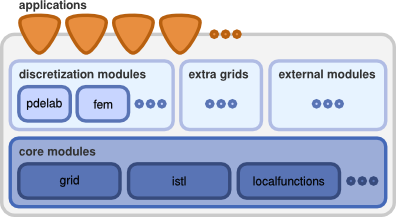
\includegraphics[width=.5\linewidth, keepaspectratio]{png/dunedesign.png}
  \caption{
    \label{fig:dune-design}
    A high-level overview of \Dune's design is available on the project's
    web site~\cite{DUNE-HP}.
  }
\end{figure}

DUNE's grid interface is independent of the spatial dimension of the
underlying grid. For this purpose, it uses the concept of
co-dimensional entities. Roughly speaking, an entity of co-dimension
$0$ constitutes a cell, co-dimension $1$ entities are faces between
cells, co-dimension $2$ are edges, and so on until co-dimension $n$
which are the cell's vertices.  The \Dune grid interface generally
assumes that all entities are convex polytopes, which means that it
must be possible to express each entity as the convex hull of a set of
vertices. For the sake of efficiency, all entities are further expressed in terms
of so-called reference elements which are transformed to the actual
spatial incarnation within the grid by a so-called geometry
function. Here, a reference element for an
entity can be thought of as a prototype for the actual grid
entity. For example, if we used a grid which applied hexahedrons as cells,
the reference element for each cell would be the unit cube $[0, 1]^3$
and the geometry function would scale and translate the cube so that
it matches the grid's cell. A quick overview of reference elements and the
related numbering can be obtained from the DUNE cheat sheet
(\url{https://www.dune-project.org/pdf/dune-cheat-sheet.pdf}).
For a more thorough description of \Dune's
grid definition, see~\cite{BASTIAN2008}.

In addition to the grid interface, \Dune also provides quite a few
additional modules, of which the \texttt{dune-localfunctions} and
\texttt{dune-istl} modules are the most relevant in the context of
this handbook. \texttt{dune-localfunctions} provides a set of generic
finite element shape functions, while \texttt{dune-istl} is the
\textbf{I}terative \textbf{S}olver \textbf{T}emplate \textbf{L}ibrary
and provides generic, highly optimized linear algebra routines for
solving the generated systems.

\Dumux comes in form of an additional module \texttt{dumux}.
It depends on the \Dune core modules
\texttt{dune-common}, \texttt{dune-grid}, \texttt{dune-istl}, and \texttt{dune-localfunctions}.
The main intention of \Dumux is to provide a framework for an easy and efficient
implementation of new physical models for porous media flow problems,
ranging from problem formulation and the selection of
spatial and temporal discretization schemes as well as nonlinear solvers,
to general concepts for model coupling.
Moreover, \Dumux includes ready to use numerical models and a few example applications.

This is the handbook to a new minor version update of \Dumux: version 3.1.
The release contains improvements and new features compared to the 3.0 version.
The update is  backwards compatible with the last release 3.0.
To facilitate the transition for our users, we have created a changelog
helping to update programs from version 3.0 to version 3.1, and giving an overview over new capabilities.
It is available online:
\url{https://git.iws.uni-stuttgart.de/dumux-repositories/dumux/blob/master/CHANGELOG.md}.
We highly recommend all our users to transition with us to the most recent version of \Dumux
and wish everyone a brand-new and exciting simulation experience.


\chapter{Quick Start}\label{quick-install}
In this chapter we provide a quick start guide to
your first \Dumux experience, including an install script with all necessary instructions
on how to very quickly install the latest release version of \Dumux.
You should have a recent working Linux environment.
If you need more information, please have a look at the detailed installation
instructions in chapter \ref{detailed-install}.
\section{Prerequisites} \label{sec:prerequisites}
For this quick start guide the following software packages are required:
\begin{itemize}
\item GitLab client
\item A standard compliant C++ compiler supporting C++11 and the C++14 feature set of GCC 4.9. We support GCC 4.9 or newer and Clang 3.8 or newer.
\item CMake 2.8.12 or newer
\item pkg-config
\item ParaView (to visualize the results)
\end{itemize}

\section{Obtaining code and configuring all modules with a script}
We provide you with a shell-script \texttt{installDumux.sh} that facilitates setting up a {\Dune}/{\Dumux} directory tree
and configures all modules with CMake.
Copy the following lines into a text file named \texttt{installDumux.sh}:
\lstinputlisting[style=DumuxCode, numbersep=5pt, firstline=1, firstnumber=1]{installDumux.sh}

Place the \texttt{installDumux.sh} script in the directory where you want to install \Dumux and \Dune (a single
root folder \texttt{DUMUX} will be produced, so you do not need to provide one). Make \texttt{installDumux.sh} executable and run the script by typing into the terminal: \texttt{./installDumux.sh}

Configuring \Dune and \Dumux is done by the command-line script \texttt{dunecontrol}
using optimized configure options, see the line entitled \texttt{\# run build} in the \texttt{installDumux.sh} script.
More details about the build-system can be found in section \ref{buildIt}.

\subsection{A first test run of \Dumux}
When the \texttt{installDumux.sh} script from the subsection above has run successfully, you can execute a second script that
will compile and run a simple one-phase ground water flow example and will visualize the result using ParaView.
The test script can be obtained by copying the following lines into a text file named \texttt{test\_dumux.sh}
that has to be located in the same directory as the installation script.
\begin{lstlisting}[style=DumuxCode]
cd DUMUX/dumux/build-cmake/test/porousmediumflow/1p/implicit/isothermal
make -B test_1p_tpfa
./test_1p_tpfa params.input
paraview *pvd
\end{lstlisting}
After making \texttt{test\_dumux.sh} executable, it can be executed by typing into the terminal: \texttt{./test\_dumux.sh}.
If everything works fine, a ParaView window with the result should open automatically, showing the initial
conditions. Advance ParaView to the next frame (green arrow button) and rescale to data range (green double arrow on top right) to admire
the colorful pressure distribution.


\chapter{Detailed Installation, Documentation, and Externals}\label{detailed-install}
In this chapter, we provide more detailed information on how to obtain source code, build and test \Dune and \Dumux.
It further contains information on
how to build the documentation and about external libraries and modules.
Installing \Dumux means that you first unpack \Dune and \Dumux in a root directory,
(section \ref{sc:ObtainingSourceCode}).
In a second step of the installation, all modules are configured with CMake
(section \ref{buildIt}).
After successful installation of \Dumux, we guide you to start a test application,
described in section \ref{quick-start-guide}.
In section \ref{sec:build-doc}, we explain how to build the \Dumux documentation.
Lastly, section \ref{sec:external-modules-libraries} provides details on optional libraries and modules.

In a technical sense \Dumux is a module of \Dune.
Thus, the installation procedure of \Dumux is the same as that of \Dune.
Details regarding the installation of \Dune are provided on the \Dune website \cite{DUNE-HP}.


\section{Obtaining Source Code for \Dune and \Dumux}
\label{sc:ObtainingSourceCode}
The \Dumux release and trunk (developer tree) are based on the most recent
\Dune release 2.7, comprising the core modules \texttt{dune-common}, \texttt{dune-geometry},
\texttt{dune-grid}, \texttt{dune-istl} and \texttt{dune-localfunctions}.
For working with \Dumux, these modules are required.
All \Dune modules, including the \Dumux module, get extracted into a common root directory, as it
is done in an ordinary \Dune installation.
We usually name our root directory \texttt{DUMUX} but an arbitrary name can be chosen.
Source code files for each \Dune module are contained in their own sub-directory within the root directory.
The sub-directories for the modules are named after the module names (depending on how
the modules were obtained, a version number is added to the module name).
The name of each \Dune module is defined in the file \texttt{dune.module}, which is
in the root directory of the respective module. This should not be changed by the user.

In section \ref{sec:prerequisites}, we list some prerequisites for running \Dune and \Dumux.
Please check in said paragraph whether you can fulfill them before continuing.

\paragraph{Obtaining \Dune and \Dumux from software repositories}
\Dune and \Dumux use Git for their software repositories. To access them,
you need to have a working installation of the version control software Git.

In the jargon of Git, \emph{cloning a certain software version} means nothing more then fetching
a local copy from the software repository and laying it out in the file system.
In addition to the software, some more files for the use of the software revision
control system itself are created. (If you have developer access to \Dumux, it is
also possible to do the opposite, i.\,e. to load up a modified revision of software
into the software repository. This is usually termed as \emph{commit} and \emph{push}.)

The download procedure is done as follows:
Create a common root directory, named e.g. \texttt{DUMUX} in the lines below.
Then, enter the previously created directory and check out the desired modules.
As you see below, the check-out uses two different servers for getting the sources,
one for \Dune and one for \Dumux.

\begin{lstlisting}[style=Bash,escapechar=\%]
$ mkdir DUMUX
$ cd DUMUX
$ git clone -b releases/2.7 https://gitlab.dune-project.org/core/dune-common.git
$ git clone -b releases/2.7 https://gitlab.dune-project.org/core/dune-geometry.git
$ git clone -b releases/2.7 https://gitlab.dune-project.org/core/dune-grid.git
$ git clone -b releases/2.7 https://gitlab.dune-project.org/core/dune-istl.git
$ git clone -b releases/2.7 https://gitlab.dune-project.org/core/dune-localfunctions.git
$ git clone -b releases/%\DumuxVersion% https://git.iws.uni-stuttgart.de/dumux-repositories/dumux.git
\end{lstlisting}

The newest and maybe unstable developments of \Dune and \Dumux are also provided in these repositories and can be found in the \emph{master} branch.
Please check the \Dune website \cite{DUNE-HP} for further information on the \Dune development. We always try to keep up with the latest developments of \Dune.
However, the current \Dumux release is based on the stable 2.7 release and it might not compile without further adaptations using the newest versions of \Dune.

Furthermore, if you wish to install the optional \Dune Grid-Howto, which provides a tutorial
on the Dune grid interface, act similar.

%TODO:currently, no DUNE patches necessary! Uncomment this section in case this changes again in the future.
%
% \paragraph{Patching \Dune or external libraries}
% \label{sc:patchingDUNE}
% Patching of \Dune modules in order to work together with \Dumux can be necessary for several reasons.
% Software like a compiler or even a standard library
% changes at times. But, for example, a certain release of a software component that we depend on,
% may not reflect that change and thus it has to be modified.
% In the dynamic developing process of software which depends on other modules it is not always feasible
% to adapt everything to the most recent version of each module. They may fix problems with a certain module
% of a certain release without introducing too much structural change.
%
% \Dumux contains patches and documentation about their usage and application within the
% directory \texttt{dumux/patches}.
% Please check the README file in that directory for recent information.
% In general, a patch can be applied as follows
% (the exact command or the used parameters may be slightly different).
% We include here an example of a patching dune-grid.
%
% \begin{lstlisting}[style=Bash]
% $ # make sure you are in the common root directory
% $ cd dune-grid
% $ patch -p0 < ../dumux/patches/grid-2.3.1.patch
% \end{lstlisting}
%
% It can be removed by
% \begin{lstlisting}[style=Bash]
% $ path -p0 -R < ../dumux/patches/grid-2.3.1.patch
% \end{lstlisting}

\section{Building \Dune and \Dumux}
\label{buildIt}
Configuring \Dune and \Dumux is done by the shell-command \texttt{dunecontrol} which is part of the \Dune build system.
If you are interested in more details about the build system that is used,
they can be found in the \Dune build system documentation\footnote{\url{https://www.dune-project.org/buildsystem/}} and
CMake's documentation\footnote{\url{https://cmake.org/documentation/}}.
If something fails during the execution of \texttt{dunecontrol}, feel free to report it to the \Dune or \Dumux developer mailing list,
but please include error details.

It is possible to compile \Dumux with nearly no explicit options to the build system.
However, for the successful compilation of \Dune and \Dumux, it is currently necessary to pass
the option \texttt{-fno-strict-aliasing} to the \Cplusplus compiler,
which is done here via a command-line argument to \texttt{dunecontrol}:
\begin{lstlisting}[style=Bash]
$ # make sure you are in the common root directory
$ ./dune-common/bin/dunecontrol --configure-opts="CXXFLAGS=-fno-strict-aliasing" --use-cmake all
\end{lstlisting}

Too many options within the command line can make life hard. That's why usually option files are being used together with \texttt{dunecontrol} and its sub-tools.
Larger sets of options are kept in them. If you are going to compile with modified options, the following
can be a starting point:
\begin{lstlisting}[style=Bash]
$ # make sure you are in the common root directory
$ cp dumux/cmake.opts my-cmake.opts      # create a personal version
$ gedit my-cmake.opts                    # optional editing the options file
$ ./dune-common/bin/dunecontrol --opts=my-cmake.opts all
\end{lstlisting}

Sometimes, it is necessary to have additional options which
are specific to a package set of an operating system or
sometimes you have your own preferences.
Feel free to work with your own set of options, which may evolve over time.
The option file that comes with the distribution is to be understood more as a starting point
for setting up an own customization than as something which is fixed.
The use of external libraries can make it necessary to add quite many options in an option file.
It can be helpful to give your customized option file its own name, as done above,
to avoid confusing it with the option files which came out of the distribution.

\section{The First Run of a Test Application}
\label{quick-start-guide}
The previous section showed how to install and compile \Dumux. This section
shall give a very brief introduction how to run a first test application and how
to visualize the first output files.\par
All executables are compiled in the \texttt{build} sub-directories of \Dumux.
If not specified differently in the options file, this is \texttt{build-cmake} as default.

\begin{enumerate}
\item Enter the folder \texttt{test/porousmediumflow/2p/implicit/incompressible} within your build directory.\\ Type \texttt{make test{\_}2p{\_}incompressible{\_}tpfa}
      in order to compile the application\\\texttt{test{\_}2p{\_}incompressible{\_}tpfa}. To run the simulation,
      type \texttt{./test{\_}2p{\_}incompressible{\_}tpfa params.input}
      into the console.
      The added \texttt{params.input} specifies that all
      important run-time parameters (like first time step size, end of simulation and location
      of the grid file) can be found in a text file in the same directory  with the
      name \texttt{params.input}.
\item The simulation starts and produces some VTU output files and also a PVD
      file. The PVD file can be used to examine time series and summarizes the VTU
      files. It is possible to stop a running application by pressing $<$Ctrl$><$c$>$.
\item You can display the results using the visualization tool ParaView (or
      alternatively VisIt). Just type \texttt{paraview} in the console and open the
      PVD file. On the upper left hand side, you can choose the desired parameter to be displayed.
\end{enumerate}

\section{Building Documentation}
\label{sec:build-doc}
Building the included documentation like this handbook requires \LaTeX{} and the auxiliary tool
\texttt{bibtex}. One usually chooses a \LaTeX{} distribution like \texttt{texlive} for this purpose.
It is possible to switch off building the documentation by setting the switch \texttt{--disable-documentation}
in the \texttt{CONFIGURE\_FLAGS} of the building options, see section \ref{buildIt}.

\subsection{Doxygen}
\label{sec:build-doxy-doc}
Doxygen documentation is done by specifically formatted comments integrated in the source code,
which can get extracted by the program \texttt{doxygen}. Beside extracting these comments,
\texttt{doxygen} builds up a web-browsable code-structure documentation
like class hierarchy of code displayed as graphs, see \url{http://www.stack.nl/~dimitri/doxygen/}.

The Doxygen documentation of a module can be built if \texttt{doxygen} is installed,
by running \texttt{dunecontrol}, entering the \texttt{build-*}directory, and executing
\texttt{make doc}. Then point your web browser to the file
\texttt{MODULE\_BUILD\_DIRECTORY/doc/doxygen/html/index.html} to read the generated documentation.
This should also work for other \Dune modules.

\subsection{Handbook}
To build the \Dumux handbook go into the \texttt{build-}directory and
run \texttt{make doc} or \texttt{make doc\_handbook\_0\_\\dumux-handbook\_pdf}. The pdf can then be found
in \texttt{MODULE\_BUILD\_DIRECTORY/doc/handbook/0\_dumux\\-handbook.pdf}.

\section{External Libraries and Modules} \label{sec:external-modules-libraries}
The libraries described below provide additional functionality but are not generally required to run \Dumux.
If you are going to use an external library, check the information provided on the \Dune website%
\footnote{DUNE: External libraries, \url{https://www.dune-project.org/doc/external-libraries/}}.
If you are going to use an external \Dune module, the website on external modules%
\footnote{DUNE: External modules, \url{https://www.dune-project.org/groups/external/}}
can be helpful.

Installing an external library can require additional libraries which are also used by \Dune.
For some libraries, such as BLAS or MPI, multiple versions can be installed on the system.
Make sure that it uses the same library as \Dune when configuring the external library.

Some of the libraries are then compiled within that directory and are not installed in
a different place, but \Dune may need to know their location. Thus, one may have to refer to
them as options for \texttt{dunecontrol}, for example via the options file \texttt{my-cmake.opts}.
Make sure you compile the required external libraries before you run \texttt{dunecontrol}.

An easy way to install some of the libraries and modules given below is the
\texttt{installexternal.sh} script located in \texttt{bin}. The script
has to be called from your common root directory.


\subsection{List of External Libraries and Modules}
\label{sec:listofexternallibs}

In the following list, you can find some external modules and external libraries,
and some more libraries and tools which are prerequisites for their use.

\begin{itemize}
\item \textbf{dune-ALUGrid}: Grid library, comes as a \Dune module.
  The parallel version needs also a graph partitioner, such as {ParMETIS}.
  Download: \url{https://gitlab.dune-project.org/extensions/dune-alugrid}

\item \textbf{dune-foamgrid}: External grid module. One- and two-dimensional grids
  in a physical space of arbitrary dimension; non-manifold grids, growth, element
  paramterizations, and movable vertices. This makes FoamGrid the grid data structure
  of choice for simulating structures such as foams, discrete fracture networks,
  or network flow problems.
  Download: \url{https://gitlab.dune-project.org/extensions/dune-foamgrid}

\item \textbf{opm-grid}: opm-grid is a DUNE module supporting grids in a corner-point format.
  Download: \url{https://github.com/OPM/opm-grid.git}

\item \textbf{dune-subgrid}: The dune-subgrid module is a meta-grid implementation that allows
to mark elements of another hierarchical dune grid and use this sub-grid just like a regular grid.
The set of marked elements can then be accessed as a hierarchical dune grid in its own right.
Dune-Subgrid provides the full grid interface including adaptive mesh refinement.
  Download: \url{https://git.imp.fu-berlin.de/agnumpde/dune-subgrid.git}

\item \textbf{dune-spgrid}: The DUNE module dune-spgrid provides a structured, parallel grid
and supports periodic boundary conditions.
  Download: \url{https://gitlab.dune-project.org/extensions/dune-spgrid.git}

\item \textbf{SuperLU}: External library for solving linear equations. SuperLU is a general purpose
  library for the direct solution of large, sparse, non-symmetric systems of linear equations.
  Download: \url{http://crd.lbl.gov/~xiaoye/SuperLU}

\item \textbf{UMFPack}: External library for solving linear equations. It is part of SuiteSparse.
  See: \url{http://faculty.cse.tamu.edu/davis/suitesparse.html}. On Debian/Ubuntu you can install the package \texttt{libsuitesparse-dev}.

\item \textbf{dune-UG}: External library for use as grid. UG is a toolbox for unstructured grids, released under GPL.
  To build UG the tools \texttt{lex}/\texttt{yacc} or the GNU variants of \texttt{flex}/\texttt{bison} must be provided.
  Download: \url{https://gitlab.dune-project.org/staging/dune-uggrid}
\end{itemize}

The following are dependencies of some of the used libraries. You will need them
depending on which modules of \Dune and which external libraries you use.

\begin{itemize}
\item \textbf{MPI}: The parallel version of \Dune and also some of the external dependencies need MPI
  when they are going to be built for parallel computing. \texttt{OpenMPI} and \texttt{MPICH} in a recent
  version have been reported to work.

\item \textbf{BLAS}: SuperLU makes use of BLAS. Thus install GotoBLAS2, ATLAS, non-optimized BLAS
  or BLAS provided by a chip manufacturer. Take care that the installation scripts select the intended
  version of BLAS.

\item \textbf{METIS} and \textbf{ParMETIS}: This are dependencies of ALUGrid and can be used with UG, if run in parallel.

\item \textbf{Compilers}: Beside \texttt{g++}, \Dune can be built with Clang from the LLVM project and
  Intel \Cplusplus compiler. C and Fortran compilers are needed for some external libraries. As code of
  different compilers is linked together, they have to be be compatible with each other.
\end{itemize}

\section{Backwards Compatibility}
\label{sec:backwardscompatibility}

Dumux Releases are split into major (e.g. 2.0, 3.0) and minor (e.g. 3.1, 3.2, 3.3) releases.
Major releases are not required to maintain backwards compatibility, 
but would provide a detailed guide on how to update dependent modules.
For each minor release, maintaining backwards compatibility is strongly encouraged and recommended.

Maintaining backwards compatibility means for all changes made to the dumux master, each tests and all dumux dependent modules should still compile. In addition, the user should be warned at compile time of any relevant interface changes. This can be done by deprecating the old method with a deprecation message and forwarding it to the new method. Examples of this are shown in the \href{https://git.iws.uni-stuttgart.de/dumux-repositories/dumux/blob/master/CONTRIBUTING.md}{contribution guide}. Each of these deprecation messages should also include the release in which the interface will be removed, and all changes should be documented thoroughly in the \href{https://git.iws.uni-stuttgart.de/dumux-repositories/dumux/-/blob/master/CHANGELOG.md}{changelog.md}.

Despite the goal of maintaining backwards compatibility across minor releases,
for more complicated changes, this is to be decided upon on a case-by-case basis, due to limited developer resources.
In the case that implementing full backwards compatibility for an update is not feasible, or would require unreasonable resources, the degree of backwards compatibility will be decided by a vote in one of the monthly core developer meetings.


\chapter{Learning to use \Dumux}\label{chp:tutorial}
So, you've downloaded your very own copy of \Dumux and its dependencies.
You've run dunecontrol, and your example ``test$\_$dumux" not only compiles,
but it even shows a nice simulation in ParaView.
Maybe you've read through parts of the handbook, and even started looking
through the Doxygen documentation.
Well done. What now? \par
%
\textit{``How on earth is this going to help me solve my multi-(phase, component,
  scale, physics) flow and transport problems in porous media systems?''}, you begin to wonder.
Don't panic! In order to best ease our prospective users and developers into the
wonderful \Dumux simulation environment, we've prepared a \Dumux course and extensively-documented examples.
\section{Hands-on \Dumux experience -- the \Dumux course}
This course is offered once a year over a period of 3 days at the University of Stuttgart.
If you're looking for information on attending, subscribe to the \Dumux mailing list
and stay tuned for updates:
\url{https://listserv.uni-stuttgart.de/mailman/listinfo/dumux}. \par
%
\textit{``But the course won't take place for another 6 months!"} and,
\textit{``I want to start developing a numerical model of my challenging and
  interesting process now!"}, you think.
Not a problem. The course materials are all shared online in their own
git repository. A series of beginner-level exercises are explained
such that you can see how a model is developed in \Dumux. As a teaser, we've
 also included a suite of examples from hot topics we're working on. Models
  exploring ``Coupling free flow and porous-media flow", ``Flow in fractured
   porous media" and ``Fluid-solid phase change" are all introduced.  \par
 %
\textit{``Sounds great, but where is this material? I can't find it within
what I've downloaded."}, you question.
The \Dumux course material is available online:
\url{https://git.iws.uni-stuttgart.de/dumux-repositories/dumux-course}. \par
In order to download this repository, which acts as an additional module to
the \Dumux base, you can download an installation script with the following command:
\begin{lstlisting}[style=Bash,escapechar=\%]
$ wget https://git.iws.uni-stuttgart.de/dumux-repositories/dumux-course/raw/releases/%\DumuxVersion%/scripts/install.sh
\end{lstlisting}
This script will install \texttt{dumux}, it's Dune dependencies, and the \texttt{dumux-course}
repository. Within the directory \texttt{dumux-course} there are a series of exercises
and slides describing the previously described examples. The course can also be added to your existing 
dumux installation using the \texttt{installExternal.py} script and the argument \texttt{course}.\par
%
The \Dumux course will be updated with each \Dumux release.
The above script will download the correct version (\textbf{releases/\DumuxVersion}) of both
the \texttt{dumux} and \texttt{dumux-course} module.

\section{Experience \Dumux by reading -- the \Dumux examples}
As an alternative to going through exercises, you can have a look at our well-documented \Dumux examples. They show how to apply \Dumux to typical physical problems. In the \texttt{README.md} files, the setup is explained, the used code is presented and documented and images resulting from the simulation are included. The \texttt{README.md} files are located directly in the subfolders of \texttt{examples} and can be displayed by web browsers.

We currently have the examples
\begin{itemize}
	\item \texttt{1ptracer}: one-phase groundwater flow including a tracer
	\item \texttt{2pinfiltration}: two-phase infiltration problem
	\item \texttt{shallowwaterfriction}: steady subcritical shallow water flow including bottom friction  
\end{itemize}
The number of examples is continuously growing.
\section{Further Practice}
\label{tutorial-furtherpractice}

If there is a need for further practice, we refer here to the test problems that
are already implemented in \Dumux. Several examples for all models
can be found in the \texttt{test}-directory. An overview over the available test
cases can be found in the class documentation \url{http://www.dumux.org/documentation.php}.

Another possibility to gain more experience with \Dumux is the \texttt{dumux-lecture} module
that contains different application examples that are used in the lectures at the
Department of Hydromechanics and Modelling of Hydrosystems in Stuttgart.
The \texttt{dumux-lecture} module can be obtained as follows:
\begin{lstlisting}[style=Bash]
$ git clone https://git.iws.uni-stuttgart.de/dumux-repositories/dumux-lecture.git
\end{lstlisting}

The module is structured based on the different lectures:
\begin{itemize}
\item mm: Multiphase Modelling,
\item efm: Environmental Fluid Mechanics,
\item mhs: Modelling of Hydrosystems.
\end{itemize}
The majority of applications is covered in the course Multiphase Modelling (mm),
while there are also some basic examples in the
courses Environmental Fluid Mechanics (efm) and Modelling of Hydrosystems (mhs).
These applications are primarily designed to enhance the understanding of conceptualizing the
governing physical processes and their implementation in a numerical simulator.
Different aspects of modeling multi-phase multi-component flow and transport processes are shown.
The lectures focus on questions like the assignment of boundary conditions, the choice of the
appropriate physics for a given problem (which phases, which components), discretization issues,
time stepping. You can find, e. g., a comparison of different two-phase flow problems: The
simpler approach considers two immiscible fluids while components in both phases with inter-phase
mass transfer are considered in the more complex approach.
All scenarios and their physical background are explained in additional .tex-files,
which are provided in sub-directories named \texttt{description}. The following test cases are
contained in the \texttt{dumux-lecture} module:
\begin{itemize}
\item \texttt{buckleyleverett}: The Buckley-Leverett Problem is a classical porous media flow show case
\item \texttt{co2plume}: Analysis of the influence of the gravitational number on a $\text{CO}_2$ plume
\item \texttt{columnxylene}: An experiment of the Research Facility for Subsurface Remediation, University of Stuttgart
\item \texttt{convectivemixing}: A test case related to CO$_2$ storage
\item \texttt{fractures}: Two-phase flow in fractured porous media
\item \texttt{fuelcell}: Water management in PEM fuel cells 
\item \texttt{heatpipe}: A show case for two-phase two-component flow with heat fluxes
\item \texttt{heavyoil}: Steam assisted gravity drainage (SAGD)
\item \texttt{henryproblem}: A show case related to salt water intrusion
\item \texttt{mcwhorter}: The McWhorter Problem is a classical porous media flow show case
\item \texttt{naplinfiltration}: Infiltration of non-aqueous phase liquid (NAPL) into soil
\item \texttt{remediationscenarios}: Test case for NAPL contaminated unsaturated soils
\item \texttt{groundwater}: Simple groundwater flow case for the course Modelling of Hydrosystems (mhs)
\item Different single/two-phase, single/two-component problems: Examples from the course Environmental Fluid Mechanics (efm)
\end{itemize}


\chapter{Overview and Infrastructure}
This chapter provides an overview of the general structure in \Dumux (\ref{sc_structure})
and gives help for basic work with \Dumux
(\ref{sc_newfoldersetup}-\ref{sc_developingdumux}).
Further it presents useful external tools (\ref{sc_externaltools}) and basic
concepts (\ref{sc_linearsystem}).
% SPDX-FileCopyrightInfo: Copyright © DuMux Project contributors, see AUTHORS.md in root folder
% SPDX-License-Identifier: CC-BY-4.0

\section{Directory Structure}
\label{sc_structure}

\Dumux has the following folder structure, which is similar to other \Dune modules.
\begin{itemize}
\item \texttt{bin}: binaries, e.g. used for the automatic testing, post-processing, installation
\item \texttt{cmake}: the configuration options for building \Dumux
\item \texttt{doc}: files necessary for the Doxygen documentation and this handbook, and various logos
\item \texttt{dumux}: the main folder, containing the source files. See Fig. \ref{fig:dumux-structure}
      for a visualized structure. For more information on the models, have a look at the
      Doxygen documentation.
\item \texttt{examples}: well-documented examples of applying \Dumux to typical physical problems. In the \texttt{README.md} files, the setup is explained, the used code is presented as well as documented and images resulting from the simulation are included. The \texttt{README.md} files are located directly in the subfolders of \texttt{examples} and can be displayed by web browsers.
\item \texttt{test}: tests for each numerical model and some functionality.
      The structure is equivalent to the \texttt{dumux} folder, the \texttt{references} folder
      contains solutions for the automatic testing. Each test program consist of a main file
      \texttt{main.cc}, the problem definition \texttt{*problem.hh} (specifying initial and boundary
      conditions), and an input file \texttt{params.input}.
      If necessary, spatially dependent parameters are defined in \texttt{*spatialparameters.hh}.
      For more detailed descriptions of the tests, please have a look at the Doxygen documentation.
\end{itemize}

\begin{figure}
% \begin{sidewaysfigure}
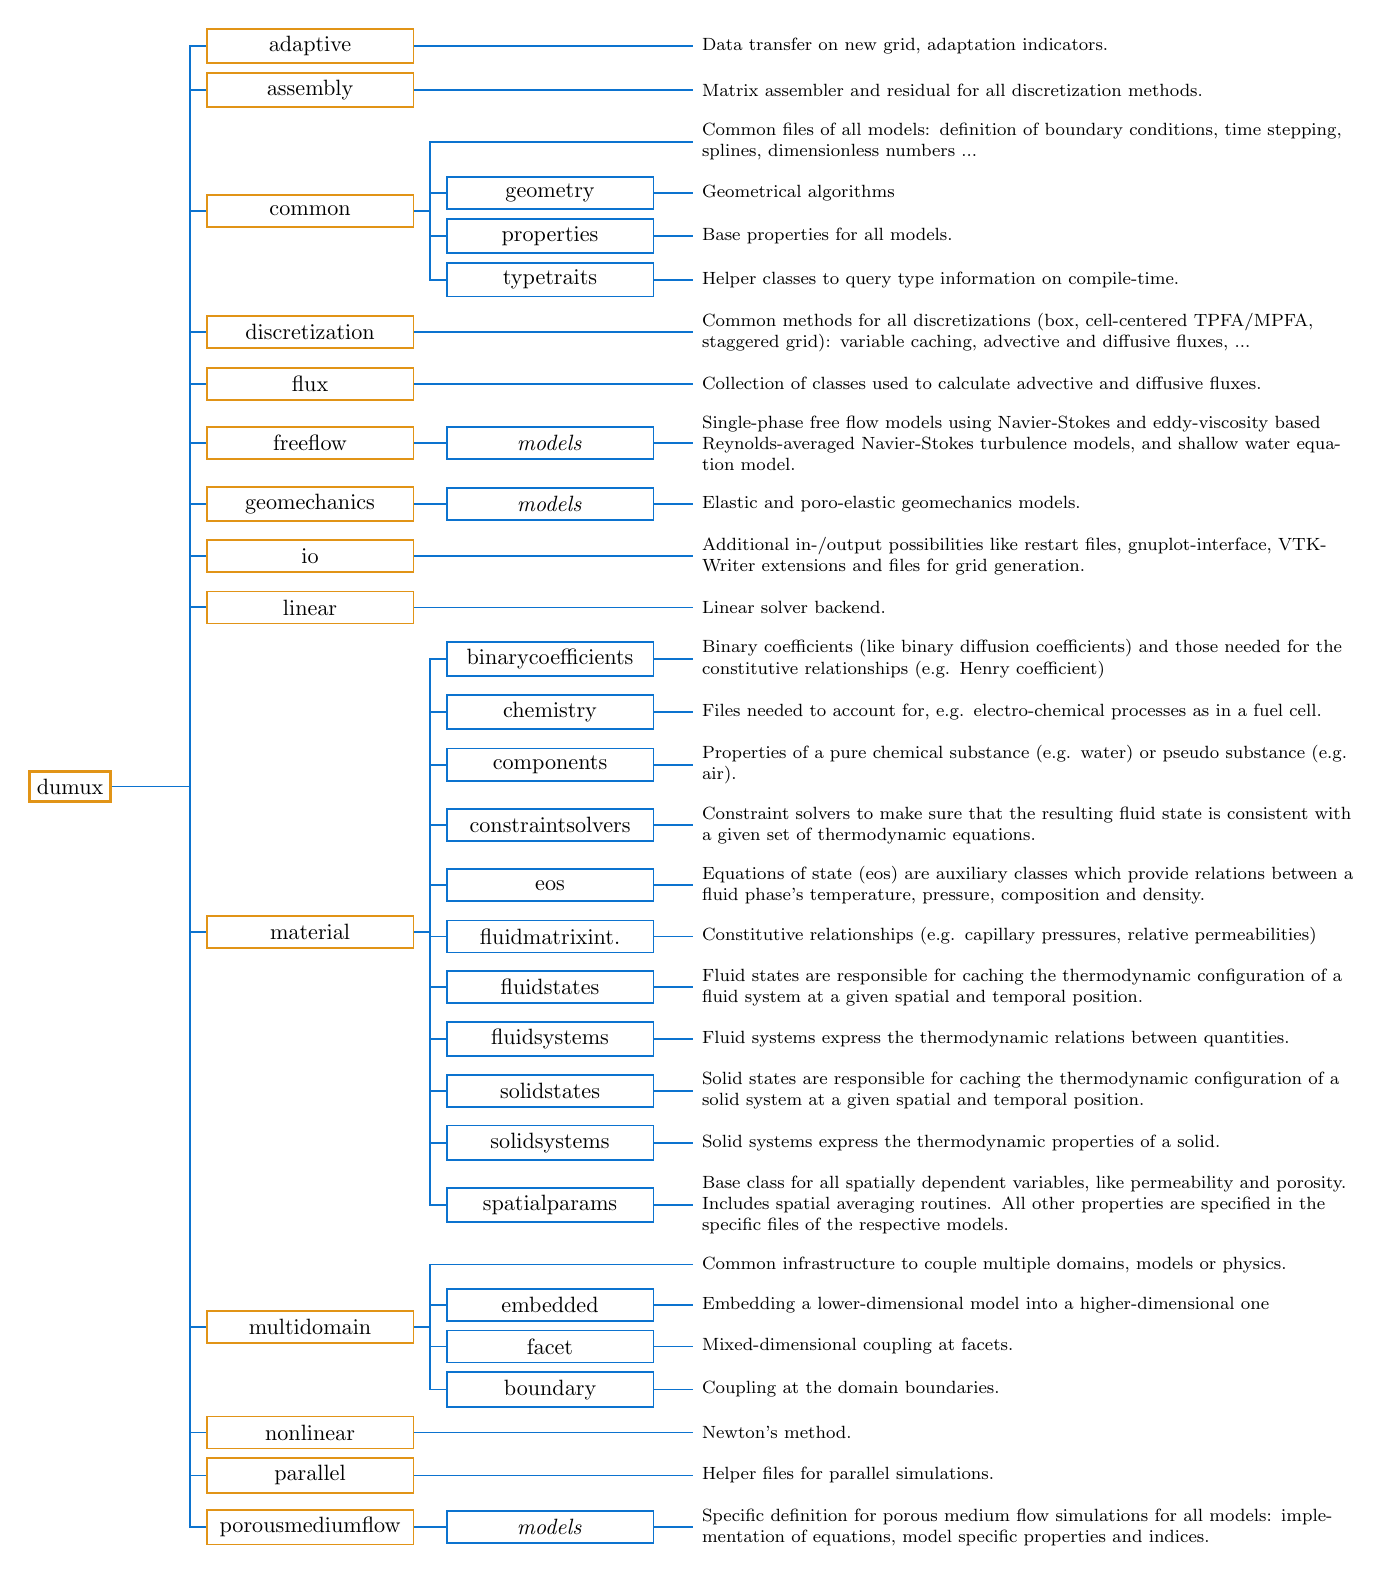
\begin{tikzpicture}[scale=0.8,grow'=right,level distance=1.5in,sibling distance=.05in]
\tikzset{edge from parent/.style={thick, draw=dumuxBlue, edge from parent fork right}}
\tikzset{every tree node/.style={draw, thick, align=center}}
\tikzset{frontier/.style={distance from root=6.0in}}

\tikzset{FirstLevel/.style={
  draw=dumuxYellow,
  rectangle,
  align=center,
  minimum width=1.1in,
  minimum height=0.2in,
  text width=1.2in,
}}
\tikzset{SecondLevel/.style={
  draw=dumuxBlue,
  rectangle,
  align=center,
  minimum width=1.1in,
  minimum height=0.2in,
  text width=1.2in,
}}

\tikzset{ThirdLevel/.style={
  draw=none,
  align=left,
  minimum width=4.2in,
  text width=4.1in,
  font=\footnotesize
}}


\Tree
[.\node[draw=dumuxYellow, ultra thick] {dumux};
  [.\node[FirstLevel] {adaptive};
    \node[ThirdLevel] {
          Data transfer on new grid, adaptation indicators.};
  ]
  [.\node[FirstLevel] {assembly};
    \node[ThirdLevel] {
          Matrix assembler and residual for all discretization methods.};
  ]
  [.\node[FirstLevel] {common};
    \node[ThirdLevel] {
          Common files of all models:
          definition of boundary conditions, time stepping, splines, dimensionless numbers ...};
    [.\node[SecondLevel] {geometry};
      \node[ThirdLevel] {Geometrical algorithms};
    ]
    [.\node[SecondLevel] {properties};
      \node[ThirdLevel] {Base properties for all models.};
    ]
    [.\node[SecondLevel] {typetraits};
      \node[ThirdLevel] {Helper classes to query type information on compile-time. };
    ]
  ]
  [.\node[FirstLevel] {discretization};
      \node[ThirdLevel] {Common methods for all discretizations (box, cell-centered TPFA/MPFA, staggered grid): variable caching, advective and diffusive fluxes, ...};
  ]
  [.\node[FirstLevel] {flux};
    [\node[ThirdLevel] {
            Collection of classes used to calculate advective and diffusive fluxes.};
    ]
  ]
  [.\node[FirstLevel] {freeflow};
    [.\node[SecondLevel] {\emph{models}};
      \node[ThirdLevel] {Single-phase free flow models using Navier-Stokes
                         and eddy-viscosity based Reynolds-averaged Navier-Stokes turbulence models, and shallow water equation model.};
    ]
  ]
  [.\node[FirstLevel] {geomechanics};
    [.\node[SecondLevel] {\emph{models}};
      \node[ThirdLevel] {Elastic and poro-elastic geomechanics models.};
    ]
  ]
  [.\node[FirstLevel] {io};
    \node[ThirdLevel] {Additional in-/output possibilities like restart files, gnuplot-interface,
                       VTKWriter extensions and files for grid generation.};
  ]
  [.\node[FirstLevel] {linear};
    \node[ThirdLevel] {Linear solver backend.};
  ]
  [.\node[FirstLevel] {material};
    [.\node[SecondLevel] {binarycoefficients};
      \node[ThirdLevel] {Binary coefficients (like binary diffusion coefficients) and those
                         needed for the constitutive relationships (e.g. Henry coefficient)};
    ]
    [.\node[SecondLevel] {chemistry};
      \node[ThirdLevel] {Files needed to account for, e.g. electro-chemical processes as in a fuel cell.};
    ]
    [.\node[SecondLevel] {components};
      \node[ThirdLevel] {Properties of a pure chemical substance (e.g. water)
                         or pseudo substance (e.g. air).};
    ]
    [.\node[SecondLevel] {constraintsolvers};
      \node[ThirdLevel] {Constraint solvers to make sure that the resulting fluid state is consistent with a
                         given set of thermodynamic equations.};
    ]
    [.\node[SecondLevel] {eos};
      \node[ThirdLevel] {Equations of state (eos) are auxiliary classes which provide
                         relations between a fluid phase's temperature, pressure, composition
                         and density.};
    ]
    [.\node[SecondLevel] {fluidmatrixint.};
      \node[ThirdLevel] {Constitutive relationships (e.g. capillary pressures, relative permeabilities)};
    ]
    [.\node[SecondLevel] {fluidstates};
      \node[ThirdLevel] {Fluid states are responsible for caching the thermodynamic
                         configuration of a fluid system at a given spatial and temporal position.};
    ]
    [.\node[SecondLevel] {fluidsystems};
      \node[ThirdLevel] {Fluid systems express the thermodynamic relations between quantities.};
    ]
    [.\node[SecondLevel] {solidstates};
      \node[ThirdLevel] {Solid states are responsible for caching the thermodynamic
                         configuration of a solid system at a given spatial and temporal position.};
    ]
    [.\node[SecondLevel] {solidsystems};
      \node[ThirdLevel] {Solid systems express the thermodynamic properties of a solid.};
    ]
    [.\node[SecondLevel] {spatialparams};
      \node[ThirdLevel] {Base class for all spatially dependent variables, like permeability and
                         porosity. Includes spatial averaging routines. All other properties are
                         specified in the specific files of the respective models.};
    ]
  ]
  [.\node[FirstLevel] {multidomain};
    \node[ThirdLevel] {
          Common infrastructure to couple multiple domains, models or physics.};
    [.\node[SecondLevel] {embedded};
      \node[ThirdLevel] {Embedding a lower-dimensional model into a higher-dimensional one};
    ]
    [.\node[SecondLevel] {facet};
      \node[ThirdLevel] {Mixed-dimensional coupling at facets.};
    ]
    [.\node[SecondLevel] {boundary};
      \node[ThirdLevel] {Coupling at the domain boundaries.};
    ]
  ]
  [.\node[FirstLevel] {nonlinear};
    \node[ThirdLevel] {Newton's method.};
  ]
  [.\node[FirstLevel] {parallel};
    \node[ThirdLevel] {Helper files for parallel simulations.};
  ]
  [.\node[FirstLevel] {porousmediumflow};
    [.\node[SecondLevel] {\emph{models}};
    \node[ThirdLevel] {Specific definition for porous medium flow simulations for all models:
                       implementation of equations,
                       model specific properties and indices.};
    ]
  ]
]
\end{tikzpicture}
\caption{Structure of the directory \texttt{dumux} containing the \Dumux source files.}
\label{fig:dumux-structure}
% \end{sidewaysfigure}
\end{figure}

% SPDX-FileCopyrightInfo: Copyright © DuMux Project contributors, see AUTHORS.md in root folder
% SPDX-License-Identifier: CC-BY-4.0

\section{Setup of new Folders and new Tests}
\label{sc_newfoldersetup}
This section describes how to set up a new folder and how to tell
the build system there is a new one.
\paragraph{Adding new Folders}
\begin{enumerate}[1)]
 \item create new folder with content
 \item adapt the \verb+CMakeList.txt+ in the folder above by adding a line with
       \verb+add_subdirectory(NEW_FOLDER)+
 \item create a \verb+CMakeList.txt+ in the newly created folder
 \item go to your \texttt{build}-directory and type \verb+make+ to
       re-configure the system
\end{enumerate}

\paragraph{Adding new Test Programs}
\noindent To add a test use the \texttt{add\_dune\_test} macro within the \texttt{CMakeList.txt} file.
The macro can be used with a variable amount of arguments. A simple call could look like this:

\begin{lstlisting}[style=DumuxCode]
dumux_add_test(NAME my_test
               SOURCES main.cc
               CMD_ARGS my_test params.input)
\end{lstlisting}

Here, we create an executable called \texttt{my\_test} from a source file \texttt{main.cc}.
The name of the test will also be \texttt{my\_test} (has to be unique). The last argument specifies a command - here, we just run the executable \texttt{my\_test} with an input file \texttt{params.input}. For more advanced uses of
the \texttt{add\_dune\_test} macro, have a look at the \texttt{test} directory. A complete documentation is given under \url{https://www.dune-project.org/sphinx/core-2.7/}.

\section{Parameters in \Dumux}
\label{sc_parameterfiles}
Simulation parameters can be parsed to the program via a parameter file or via the command line.

After having run the example application from the getting started guide you will
get the following output at the end of the simulation run
\footnote{If you did not get the output, add \texttt{Parameters::print();} to your main file.}:
\begin{lstlisting}[style=Bash]
# Runtime-specified parameters used:
[ Grid ]
Cells = "48 32"
UpperRight = "6 4"
[ Newton ]
EnablePartialReassembly = "true"
[ Problem ]
EnableGravity = "true"
Name = "2p"
[ SpatialParams ]
LensLowerLeft = "1.0 2.0"
LensUpperRight = "4.0 3.0"
[ TimeLoop ]
DtInitial = "250"
TEnd = "3000"

# Global default parameters used:
[ Assembly ]
NumericDifferenceMethod = "1"
[ Flux ]
UpwindWeight = "1.0"
[ LinearSolver ]
MaxIterations = "250"
ResidualReduction = "1e-13"
Verbosity = "0"
[ LinarSolver.Preconditioner ]
Iterations = "1"
Relaxation = "1.0"
[ Newton ]
EnableAbsoluteResidualCriterion = "false"
EnableChop = "false"
EnableResidualCriterion = "false"
EnableShiftCriterion = "true"
MaxAbsoluteResidual = "1e-5"
MaxRelativeShift = "1e-8"
MaxSteps = "18"
MinSteps = "2"
ResidualReduction = "1e-5"
SatisfyResidualAndShiftCriterion = "false"
TargetSteps = "10"
UseLineSearch = "false"
[ TimeLoop ]
MaxTimeStepSize = "1e300"
[ Vtk ]
AddProcessRank = "true"
AddVelocity = "false"

# Unused parameters:
Grid.LowerLeft = "0 0"
\end{lstlisting}

A number of things can be learned:
\begin{itemize}
  \item \emph{run-time} parameters can be changed without re-compiling
  \item \emph{default parameters} are set by default
  \item \emph{unused} parameters are not used by the simulation (maybe typo or wrong group in input file)
\end{itemize}


\subsection{Parameter Values}
To get the value of an input parameter please use:
\begin{lstlisting}[name=propsyscars,style=DumuxCode]
static const TYPE paramname = getParam<TYPE>("GROUPNAME.PARAMNAME");
\end{lstlisting}

If you also want to set a default value for a parameter, just add it like this:

\begin{lstlisting}[name=propsyscars,style=DumuxCode]
static const TYPE paramname = getParam<TYPE>("GROUPNAME.PARAMNAME", default);
\end{lstlisting}

As this function call is relatively expensive, the respective variables should always be \texttt{static} (e.g., if used in a loop). When dealing with multiple group names, e.g., in the context of coupled models, the following methods might be more convenient:

\begin{lstlisting}[name=propsyscars,style=DumuxCode]
auto modelParamGroup0 = "Model0";
static const TYPE paramname0 = getParamFromGroup<TYPE>(modelParamGroup0, "GROUPNAME.PARAMNAME");
auto modelParamGroup1 = "Model1";
static const TYPE paramname1 = getParamFromGroup<TYPE>(modelParamGroup1, "GROUPNAME.PARAMNAME");
\end{lstlisting}

The \texttt{FVProblem} class provides a convenience function \texttt{paramGroup()}.

The parameters can then be specified in the input file:

\begin{lstlisting}[style=Bash]
[ Model0.Grid ]
File = file0.dgf
[ Model1.Grid ]
File = file1.dgf
\end{lstlisting}

\section{Restart \Dumux Simulations}
\label{sc_restartsimulations}

\Dumux has some experimental support for check-pointing (restarting paused/stopped/crashed simulations).
You can restart a \Dumux simulation from any time point where a VTK file was written out.
This is currently only supported for sequential, non-adaptive simulations. For adaptive simulation
the full hierarchical grid has to be stored. This is usually done with the grid's \texttt{BackupRestoreFacility}.
There is currently no special support by \Dumux for that, but it is possible to implement
a restart using \texttt{BackupRestoreFacility} with plain Dune.

For VTK files the output can be read with the free function \texttt{loadSolution}. Grids can be read with
the \texttt{Dumux::VTKReader} or you can simply recreate the grid as you did in the first simulation run.

Writing double-precision floating point numbers to VTK files is available since \Dune release 2.7. If you are using that version, it is now possible to specify output precision in the input file using \texttt{Vtk.Precision} followed by either \texttt{Float32}, \texttt{Float64}, \texttt{UInt32}, \texttt{UInt8} or \texttt{Int32}. \texttt{Float32} is set as the default. We especially advice the use of \texttt{Float64} when working with restart files.

The restart capabilities will hopefully be improved in future versions of \Dumux-3.
We are looking forward to any contributions (especially HDF5 / XDMF support, improvement of VTK support).

\section{Developing \Dumux}
\label{sc_developingdumux}

\subsection{Communicate with \Dumux Developers}

\paragraph{Issues and Bug Tracking}
The bug-tracking system \emph{GitLab Issues} offers the possibility to report bugs or discuss new development requests.
Feel free to register (if you don't have an account at out \emph{Git} yet) and to contribute
at \url{https://git.iws.uni-stuttgart.de/dumux-repositories/dumux/issues}.

\paragraph{Commits, Merges, etc.}
To be up-to-date with the latest changes made to any git-repository, you can use RSS Feeds.
Simply click on \emph{Issues} or \emph{Activity} and then select a tab you are interested in
and use your favorite RSS-application for receiving the news.

\paragraph{Automatic Testing Dashboard}
The automatic testing using \emph{BuildBot} helps to constantly check the
\Dumux problems for compiling and running correctly. It is available at
\url{https://git.iws.uni-stuttgart.de/buildbot/#/builders}.

\paragraph{The General Mailing List:}
If you have questions, specific problems (which you really struggle to solve on your own),
or hints for the \Dumux-developers, please contact the mailing list \url{dumux@iws.uni-stuttgart.de}.
You can subscribe to the mailing list via
\url{https://listserv.uni-stuttgart.de/mailman/listinfo/dumux}, then you
will be informed about upcoming releases or events.

\subsection{Coding Guidelines}
Writing code in a readable manner is very important, especially
for future code developers (e.g. for adding features, debugging, etc.).
For the style guide and instructions how to contribute to \Dumux visit
\url{https://git.iws.uni-stuttgart.de/dumux-repositories/dumux/blob/master/CONTRIBUTING.md}.


\subsection{Tips and Tricks}
\Dumux users and developers at the LH2 are also referred to the internal confluence pages for
more information.

\paragraph{Optimized computation vs debugging}
\Dune and \Dumux are built with the help of \texttt{dunecontrol}, as explained on page \pageref{buildIt}.
Per default, \Dumux is compiled using optimization options, which leads to faster runtimes but is unsuitable
for debugging. For debug opts you can set \texttt{DCMAKE\textunderscore BUILD\textunderscore TYPE} to \texttt{Debug} or \texttt{RelWithDebInfo}
in your options file. You can also do this in any of the \texttt{CMakeLists.txt} in Dumux by adding:

\begin{lstlisting}[style=Shell]
set(CMAKE_BUILD_TYPE Debug)
\end{lstlisting}

Afterwards rerun cmake (run cmake \texttt{$<$path-to-build-dir$>$}).

\paragraph{Dunecontrol for selected modules}
A complete build using \texttt{dunecontrol} takes some time. In many cases not all modules need to be re-built.
Pass the flag \texttt{--only=dumux} to \texttt{dunecontrol} for configuring or building only \Dumux. A more
complex example would be a case in which you have to configure and build only e.g. \Dune{}-grid
and \Dumux. This is achieved by adding \texttt{--only=MODULE,dumux}.

\paragraph{Patching Files or Modules}
If you want to send changes to an other developer of \Dumux providing patches
can be quite smart. To create a patch simply type:
\begin{lstlisting}[style=Bash]
$ git diff > PATCHFILE
\end{lstlisting}
\noindent which creates a text file containing all your changes to the files
in the current folder or its subdirectories.
To apply a patch in the same directory type:
\begin{lstlisting}[style=Bash]
$ patch -p1 < PATCHFILE
\end{lstlisting}

%TODO: currently, no DUNE patches necessary! Thus, this section is commented and the missing refrence would be bad.
% Uncomment the following statement again when patches might be necessary.
% See \ref{sc:patchingDUNE} if you need to apply patches to \Dumux or \Dune.

\paragraph{File Name and Line Number by Predefined Macro}
If you want to create output in order to later know where some output or debug information came from, use the predefined
macros \texttt{\_\_FILE\_\_} and \texttt{\_\_LINE\_\_}:
\begin{lstlisting}[style=DumuxCode]
std::cout << "# This was written from "<< __FILE__ << ", line " << __LINE__ << std::endl;
\end{lstlisting}

\paragraph{Using \Dune Debug Streams}
\Dune provides a helpful feature for keeping your debug-output organized.
It uses simple streams like \texttt{std::cout}, but they can be switched on and off
for the whole project. You can choose five different levels of severity:
\begin{verbatim}
5 - grave (dgrave)
4 - warning (dwarn)
3 - info (dinfo)
2 - verbose (dverb)
1 - very verbose (dvverb)
\end{verbatim}
\noindent They are used as follows:
\begin{lstlisting}[style=DumuxCode]
// define the minimal debug level somewhere in your code
#define DUNE_MINIMAL_DEBUG_LEVEL 4
Dune::dgrave << "message"; // will be printed
Dune::dwarn << "message"; // will be printed
Dune::dinfo << "message"; // will NOT be printed
\end{lstlisting}

\paragraph{Make headercheck:}
To check one header file for all necessary includes to compile the contained code, use \texttt{make headercheck}.
Include the option \texttt{-DENABLE\_HEADERCHECK=1} in your opts file and run \texttt{dunecontrol}.
Then go to the top level in your build-directory and type \texttt{make headercheck} to check all headers
or press 'tab' to use the auto-completion to search for a specific header.

\section{External Tools}
\label{sc_externaltools}

\subsection{Git}
Git is a version control tool which we use.
The basic Git commands are:
\begin{itemize}
  \item \texttt{git checkout}: receive a specified branch from the repository
  \item \texttt{git clone}: clone a repository; creates a local copy
  \item \texttt{git diff}: to see the actual changes compared to your last commit
  \item \texttt{git pull}: pull changes from the repository; synchronizes the
  repository with your local copy
  \item \texttt{git push}: push comitted changes to the repository;  synchronizes
  your local copy with the repository
  \item \texttt{git status}: to check which files/folders have been changed
  \item \texttt{git gui}: graphical user interface, helps selecting changes for
  a commit
\end{itemize}


\subsection{Gnuplot}
\label{gnuplot}
A gnuplot interface is available to plot or visualize results during a simulation run.
This is achieved with the help of the \texttt{Dumux::GnuplotInterface} class provided in \texttt{io/gnuplotinterface.hh}.

To use the gnuplot interface you have to make some modifications in your file, e.g., your main file.

First, you have to include the corresponding header file for the gnuplot interface.
\begin{lstlisting}[style=DumuxCode]
#include <dumux/io/gnuplotinterface.hh
\end{lstlisting}

Second, you have to define an instance of the class \texttt{Dumux::GnuplotInterface} (e.g. called \texttt{gnuplot}).
\begin{lstlisting}[style=DumuxCode]
Dumux::GnuplotInterface<double> gnuplot;
\end{lstlisting}

As an example, to plot the mole fraction of nitrogen (\texttt{y}) over time (\texttt{x}),
extract the variables after each time step in the time loop.
The actual plotting is done using the method of the gnuplot interface:

\begin{lstlisting}[style=DumuxCode]
gnuplot.resetPlot();                             // reset the plot
gnuplot.setXRange(0.0, 72000.0);                 // specify xmin and xmax
gnuplot.setYRange(0.0, 1.0);                     // specify ymin and ymax
gnuplot.setXlabel("time [s]");                   // set xlabel
gnuplot.setYlabel("mole fraction mol/mol");  // set ylabel

// set x-values, y-values, the name of the data file and the Gnuplot options
gnuplot.addDataSetToPlot(x, y, "N2.dat", options);

gnuplot.plot("mole_fraction_N2");                // set the name of the output file
\end{lstlisting}

It is also possible to add several data sets to one plot by calling \texttt{addDataSetToPlot()} more than once.
For more information have a look into a test including the gnuplot interface header file, the doxygen documentation
of \texttt{Dumux::GnuplotInterface}, or the header file itself (\texttt{dumux/io/gnuplotinterface.hh}).


\subsection{Gstat}
Gstat is an open source software tool which generates geostatistical random fields (see \url{www.gstat.org}).
In order to use gstat, execute the \texttt{bin/installexternal.sh} from your \Dumux root
directory or donwload, unpack and install the tarball from the gstat-website.
Then, rerun cmake (in the second case set \texttt{GSTAT\_ROOT} in your input file to the
path where gstat is installed).


\subsection{ParaView}
\paragraph{Reload Button:}
There are scripts to reload PVD or series of VTU files since ParaView 4.2.
The scripts can be found
\href{http://markmail.org/message/exxynsgishbvtngg#query:+page:1+mid:rxlwxs7uqrfgibyv+state:results}{\texttt{under this link}}.
Just save the specific code portion in a file and load it via \texttt{Macros} $\rightarrow$ \texttt{Add new macro}.

\paragraph{Guide:}
Since ParaView 4.3.1, The ParaView Guide is partly
available for free download, see \url{http://www.paraview.org/documentation/}.
It contains similar content as the ParaView book.

\section{Assembling the linear system}
\label{sc_linearsystem}
The physical system is implemented as the mathematical differential equation in
local operators. \Dumux generates the linear system automatically. Read on, to
learn what is done internally.

\subsection{Newton's method}
The differential equations are implemented in the residual form. All terms are
on the left hand side and are summed up. The terms contain values for the primary
variables which are part of the solution vector $\textbf{u}$. The sum of the terms
is called residual $\textbf{r}(\textbf{u})$ which is a function of the solution. For
example:
\begin{align*}
\underbrace{
  \phi \frac{\partial \varrho_\alpha S_\alpha}{\partial t}
 -
 \text{div} \left(
 \varrho_\alpha \frac{k_{r\alpha}}{\mu_\alpha} \mathbf{K}
 \left(\grad\, p_\alpha - \varrho_{\alpha} \mathbf{g} \right)
 \right) - q_\alpha} _
{=: \, \textbf{r}(\textbf{u})}
= 0
\end{align*}

We don't know the solution $\textbf{u}$, so we use the iterative Newton's method to
obtain a good estimate of $\textbf{u}$. We start with an initial guess $\textbf{u}^0$ and
calculate it's residual $\textbf{r}(\textbf{u}^0)$. To minimize the error, we calculate
the derivative of the residual with respect to the solution. This is the Jacobian
matrix
\begin{align*}
  \frac{\text{d}}{\text{d}\textbf{u}}\textbf{r} \left(\textbf{u}^i\right)
  = J_{\textbf{r} \left(\textbf{u}^i\right)}
  = \left(\frac{\text{d}}{\text{d}\textbf{u}^i_m}\textbf{r} \left(\textbf{u}^i\right)_n\right)_{m,n}
\end{align*}
with $i$ denoting the Newton iteration step.
Each column is the residual derived with respect to the $m$th entry of $\textbf{u}^i$.

The Jacobian indicates the direction where the residual increases. By solving the
linear system
\begin{align*}
  J_{\textbf{r}(\textbf{u}^i)} \cdot \textbf{x}^i = \textbf{r}(\textbf{u}^i)
\end{align*}
we calculate the direction of maximum growth $\textbf{x}^i$. We subtract it from
our current solution to get a new, better solution
$\textbf{u}^{i+1} = \textbf{u}^i - \textbf{x}^i$.

We repeat the calculation of of the Jacobian $J_{\textbf{r}(\textbf{u}^i)}$ and the
direction of maximum growth $\textbf{x}^i$ until our approximated solution becomes good enough.

\subsection{Structure of matrix and vectors}
To understand the meaning of an entry in the matrix or the vector of the linear system, we have
to define their structure. Both have a blocking structure. Each block contains the degrees of
freedom (also called variable or unknown) for a control volume. The equation index is used
to order of the degrees of freedom. For each control volume we have one block. The mapper is
used to order the blocks.

\begin{figure}[htbp]
\begin{center}
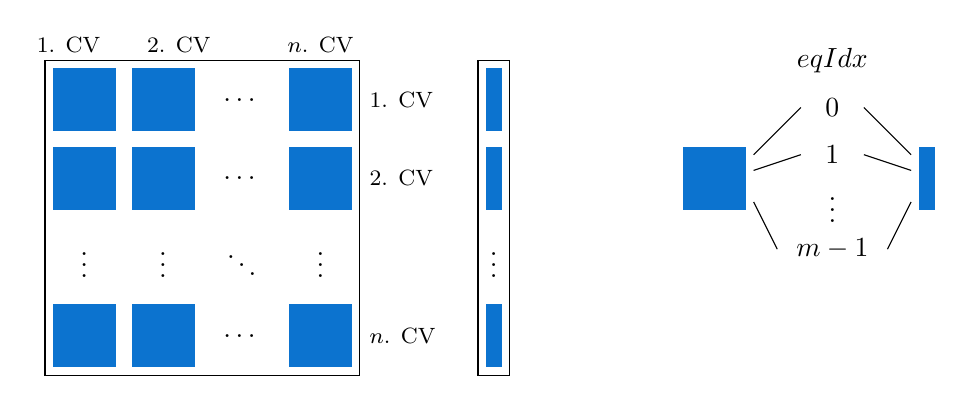
\begin{tikzpicture}[fill=dumuxBlue]
  %% blocking structure
  % matrix
  \node at (0.3,4.2){\footnotesize 1. CV};
  \node at (1.7,4.2){\footnotesize 2. CV};
  \node at (3.5,4.2){\footnotesize $n$. CV};

  \draw (0,0) rectangle (4,4);

  \fill (0.1,3.1) rectangle (0.9,3.9);
  \fill (1.1,3.1) rectangle (1.9,3.9);
  \node at (2.5,3.5) {$\dots$};
  \fill (3.1,3.1) rectangle (3.9,3.9);
  \node at (4,3.5) [right]{\footnotesize 1. CV};

  \fill (0.1,2.1) rectangle (0.9,2.9);
  \fill (1.1,2.1) rectangle (1.9,2.9);
  \node at (2.5,2.5) {$\dots$};
  \fill (3.1,2.1) rectangle (3.9,2.9);
  \node at (4,2.5) [right]{\footnotesize 2. CV};

  \node at (0.5,1.5) {$\vdots$};
  \node at (1.5,1.5) {$\vdots$};
  \node at (2.5,1.5) {$\ddots$};
  \node at (3.5,1.5) {$\vdots$};

  \fill (0.1,0.1) rectangle (0.9,0.9);
  \fill (1.1,0.1) rectangle (1.9,0.9);
  \node at (2.5,0.5) {$\dots$};
  \fill (3.1,0.1) rectangle (3.9,0.9);
  \node at (4,0.5) [right]{\footnotesize $n$. CV};

  % vector
  \draw (5.5,0) rectangle (5.9,4);
  \fill (5.6,3.1) rectangle (5.8,3.9);
  \fill (5.6,2.1) rectangle (5.8,2.9);
  \node at (5.7,1.5) {$\vdots$};
  \fill (5.6,0.1) rectangle (5.8,0.9);

  %% intra-block structure
  \fill (8.1,2.1) rectangle (8.9,2.9);
  \draw (9,2.8) -- (9.6,3.4);
  \draw (9,2.6) -- (9.6,2.8);
  \draw (9,2.2) -- (9.3,1.6);

  \node at (10,4) {${eqIdx}$};
  \node at (10,3.4) {$0$};
  \node at (10,2.8) {$1$};
  \node at (10,2.2) {$\vdots$};
  \node at (10,1.6) {$m-1$};

  \fill (11.1,2.1) rectangle (11.3,2.9);
  \draw (11,2.8) -- (10.4,3.4);
  \draw (11,2.6) -- (10.4,2.8);
  \draw (11,2.2) -- (10.7,1.6);
\end{tikzpicture}
\end{center}
\caption{Structure of matrix and vector, left blocking structure, right within block}
\end{figure}

Accessing entries follows this structure. You can access the pressure value in the third sub-control volume in
a vector \lstinline{sol} with \lstinline{sol[2][pressureIdx]}.


\chapter{Advanced \Dumux\ -- Detailed Instructions}
This chapter contains detailed information for those who are interested
in deeper modifications of underlying \Dumux models, classes, functions, etc.
% SPDX-FileCopyrightInfo: Copyright © DuMux Project contributors, see AUTHORS.md in root folder
% SPDX-License-Identifier: CC-BY-4.0

\section{Physical Basics}
Here, the basic definitions, the general models concept, and a list of
models available in \Dumux are given. The actual differential equations
can be found in the local residuals (see Doxygen documentation of the
model's \texttt{LocalResidual} class).

\subsection{Basic Definitions and Assumptions}
Basic definitions and assumptions are given. More information can be found e.g. in \cite{A3:acosta:2006,A3:bielinski:2006}.

\begin{description}
\item[Phases:]
A \emph{phase} is defined as a continuum having distinct properties (e.g. density and viscosity). If phases are miscible, they contain dissolved portions of the substance of the other phase. 
Fluid and solid phases are distinguished. The fluid phases have different affinities to the solid phases. The phase, which has a higher affinity to the solid phases is referred to as the (more) wetting phase. In the case of two phases, the less wetting one is called the nonwetting phase. 

For compositional multi-phase models, fluid phases may be composed of several components, while the solid phases are assumed to consist exclusively of a single component. 

\item[Components:]
The term \emph{component} stands for constituents of the phases which
can be associated with a unique chemical species or, more generally, with
a group of species exploiting similar physical behavior. For example, Fig. \ref{fig:phaseMassEnergyTransfer} shows a water-gas-NAPL system composed of the phases water (subscript
$\text{w}$), gas ($\text{g}$), and NAPL ($\text{n}$). These phases are
composed of the components water (superscript $\text{w}$), the pseudo-component
air ($\text{a}$), and an organic contaminant ($\text{c}$).

The composition of the components in a phase can influence the phase properties. Furthermore, for mass transfer, the phase behavior is quite different from the component behavior.

\item[Equilibrium:]
For the non-isothermal, multi-phase, multi-component processes in porous media
we state the assumption of \emph{local thermodynamic equilibrium}.
Chemical equilibrium means that the mass/mole fractions of a component in
different phases are in equilibrium.
Thermal equilibrium assumes the same temperature for all considered phases.
Mechanical equilibrium is not valid in a porous medium, since discontinuities
in pressure can occur across a fluid-fluid interface due to capillary effects.

\item[Notation:]
The subscript index $\alpha$, e.g. $\text{w}, \text{n} \text{ and } \text{g}$ in the example of Fig. \ref{fig:phaseMassEnergyTransfer}, refers
to the phase, while the superscript $\kappa$, e.g. $\text{w}, \text{a} \text{ and } \text{c}$ in the example of Fig. \ref{fig:phaseMassEnergyTransfer},
refers to the component.
\end{description}

\begin{table}
\begin{tabular}{llll}
$p_\alpha$ & phase pressure & $\phi$ & porosity \\
$T$ & temperature & $K$ & absolute permeability tensor \\
$S_\alpha$ & phase saturation & $\tau$ & tortuosity \\
$x_\alpha^\kappa$ & mole fraction of component $\kappa$ in phase $\alpha$ & $\boldsymbol{g}$ & gravitational acceleration \\
$X_\alpha^\kappa$ & mass fraction of component $\kappa$ in phase $\alpha$ & $q^\kappa_\alpha$ & volume source term of $\kappa$ in $\alpha$ \\
$\varrho_{\text{mol},\alpha}$ & molar density of phase $\alpha$ & $u_\alpha$ & specific internal energy \\
$\varrho_{\alpha}$ & mass density of phase $\alpha$ & $h_\alpha$ & specific enthalpy \\
$M$ & molar mass of a phase or component & $c_\text{s}$ & specific heat enthalpy \\
$k_{\text{r}\alpha}$ & relative permeability & $\lambda_\text{pm}$ & heat conductivity \\
$\mu_\alpha$ & phase viscosity & $q^h$ & heat source term \\
$D_\alpha^\kappa$ & diffusivity of component $\kappa$ in phase $\alpha$ & $\boldsymbol{v}_{a,\alpha}$  & advective velocity \\
$\boldsymbol{v}_\alpha$ & velocity (Darcy or free flow)& & \\
\end{tabular}
\caption{Notation list for most of the variables and indices used in \Dumux.}

\end{table}

\begin{figure}
  \centering
  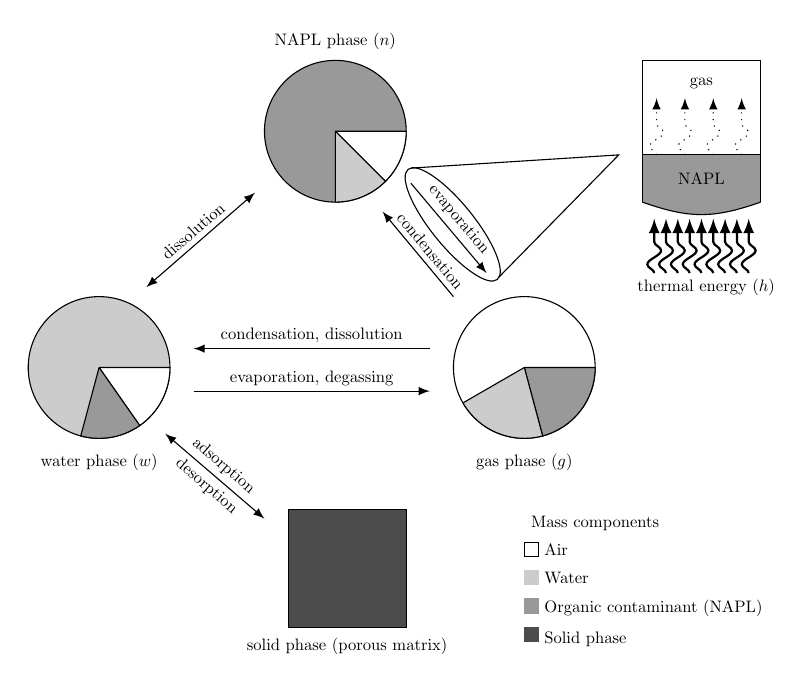
\begin{tikzpicture} [>=latex,scale=0.6, every node/.style={transform shape}]
    % Ellipse 1 solid
    \coordinate (A) at (1,-0.5);
    \draw [fill=black!70](A) rectangle(3.5,2) node at(2.25,-0.9) {solid phase (porous matrix)};
    % Ellipse 2 water
    \coordinate (B) at (-3,5);
    \draw [fill=black!20](B) circle(1.5cm);
    \node [yshift=5mm]at(-3,2.5){water phase $(w)$};
    \draw[fill=white] (B)--+(1.5,0)arc(0:-55:1.5cm)--(B);
    \draw[fill=black!40] (B)--+(-55:1.5cm)arc(-55:-105:1.5cm)--(B);
    % Ellipse 3 gas
    \coordinate (C) at (6,5);
    \draw [](C) circle (1.5cm);
    \node[yshift=5mm]at(6,2.5){gas phase $(g)$};
    \draw [fill=black!40](C)--+(1.5,0)arc(0:-75:1.5cm)--(C);
    \draw [fill=black!20] (C)--+(-75:1.5cm)arc(-75:-150:1.5cm)--(C);
    % Ellipse 4 napl
    \coordinate (D) at (2,10);
    \draw [fill=black!40](D) circle (1.5cm);
    \node[yshift=5mm]at(2,11.4){NAPL phase $(n)$};
    \draw [fill=white](D)--+(1.5,0)arc(0:-45:1.5cm)--(D);
    \draw [fill=black!20] (D)--+(0,-1.5)arc(-90:-45:1.5cm)--(D);
    % arrows
    %A-B
      \draw [<->,white](0.5,1.8)--(-1.6,3.6) node[black,above,sloped,pos=0.5]{adsorption};
      \draw [<->](0.5,1.8)--(-1.6,3.6) node[below,sloped,pos=0.5]{desorption};
    %B-C
      \draw[<-](-1,5.4)--(4,5.4)node[above,sloped,pos=0.5]{condensation, dissolution};
      \draw[->](-1,4.5)--(4,4.5)node[above,sloped,pos=0.5]{evaporation, degassing};
    %B-D
      \draw[<->](-2,6.7)--(0.3,8.7)node[above,sloped,pos=0.5]{dissolution};
    %D-C
      \draw[->](3.6,8.9)--(5.2,7)node[above,sloped,pos=0.5]{evaporation};
      \draw[rotate around={-51:(4,6.8)}](3.35,7.95) ellipse (1.5cm and 0.45cm);  %Ellipse um evaporation
      \draw (3.6,9.22)--(8,9.5)--(5.45,6.9);
      \draw[<-](3,8.3)--(4.5,6.5)node[above,sloped,pos=0.55]{condensation};
    % thermal energy
    \filldraw [black!40](8.5,9.5)rectangle(11,8.5);
    \draw (8.5,9.5)rectangle(11,11.5);
    \draw (8.5,9.5)--(8.5,8.5);
    \draw (11,9.5)--(11,8.5);
    \draw [decorate,decoration={bent,aspect=0.4,amplitude=6},fill=black!40](11,8.5)--(8.5,8.5);
    \foreach \x in {8.75,9,...,10.8}
    \draw [->,decorate,decoration={snake,post length=2mm},thick](\x,7)--(\x,8.15);
    \foreach \x in {8.8,9.4,10,10.6}
    \draw [->,dotted,decorate,decoration={snake,post length=2mm}](\x,9.5)--(\x,10.7);
    \node at(9.75,11){gas};
    \node at(9.75,9){NAPL};
    \node at(9.85,6.7){thermal energy $(h)$};
    % legende
    \node at (7.5,1.7){Mass components};
    \draw[](6,1)rectangle +(0.3,0.3) node at(6.3,1.15) [right]{Air};
    \filldraw[black!20](6,0.4) rectangle +(0.3,0.3) node at (6.3,0.55)[black,right]{Water};
    \filldraw[black!40](6,-0.2) rectangle +(0.3,0.3) node at (6.3,-0.1)[right,black]{Organic contaminant (NAPL)};
    \filldraw[black!70](6,-0.8) rectangle +(0.3,0.3) node at (6.3,-0.75)[right,black]{Solid phase};
  \end{tikzpicture}
  \caption{Mass and energy transfer between the phases in a water-NAPL-gas system \cite{A3:class:2002a}}
  \label{fig:phaseMassEnergyTransfer}
\end{figure}

\subsection[Scale]{Scale\footnote{\label{foot:hommel}This subsection is taken from \cite{hommel2016modeling} in a slightly adapted form.}} 

Depending on the scale of interest, physical and chemical processes and properties can be described 
using different approaches. 
On the molecular scale, the properties and interactions of individual molecules are described, 
which is only feasible for a restricted number of molecules. 
For larger systems, a continuum approach is used, where properties are averaged over 
groups of similar molecules, assuming continuous matter. This upscaling by averaging 
from the molecular scale results in the micro-scale, on which the system is described by
the pore geometry and the distribution of distinct fluid phases within the pores. 
However, for larger laboratory or field-scale applications, the micro-scale is still 
computationally prohibitively expensive and system descriptions on the macro-scale 
are used for calculations. The macro-scale description is obtained by averaging over the 
micro-scale properties within a representative elementary volume (REV), 
which needs to be large enough to ensure that the averaged properties are independent of the REV size 
or position. However, it should in turn be much smaller than the entire domain size \citep{helmig1997multiphase}. %(Bear 1988)
The detailed pore-geometry and phase-distribution information of the micro-scale is lost
on the macro-scale and replaced by volume average quantities, 
such as porosity, permeability and phase saturation, 
and relations like the Darcy's law.
The macro-scale is also called the REV (or Darcy) scale and is the scale of the 
models available in \Dumux.

\subsection[Porous medium properties]{Porous medium properties\footref{foot:hommel}}
\subsubsection{Porosity}
The porosity $\phi$ is defined as the fraction of the volume occupied by fluids in an REV $V_\mathrm{fluid}$ 
divided by the total volume of the REV $V_\mathrm{total}$.

\begin{equation}\label{eq:def_poro}
\phi=\frac{V_\mathrm{fluid}}{V_\mathrm{total}}=1-\frac{V_\mathrm{solid}}{V_\mathrm{total}}.
\end{equation}


\subsubsection{Intrinsic permeability} 
The intrinsic permeability is a measure on the REV scale of the ease of fluid flow through porous media. 
It relates the potential gradient and the resulting flow velocity in the Darcy equation. 
As the porous medium may have a structure leading to preferential flow in certain directions, 
intrinsic permeability is in general a tensorial quantity $\mathbf{K}$. 
For isotropic porous media, it can be reduced to a scalar quantity $K$.

% \begin{equation}
%  \mathbf{v}=
% \end{equation}

\newpage
\subsection[Mass fraction, mole fraction]{Mass fraction, mole fraction\footref{foot:hommel}}\label{sec:mole_frac_molality}
The composition of a phase is described by mass or mole fractions of the components. 
The mole fraction $x^\kappa_\alpha$ of component $\kappa$ in phase $\alpha$ is defined as:

\begin{equation}\label{eq:def_molefrac}
x^\kappa_\alpha = \frac{n^\kappa_\alpha}{\sum_i n^i_\alpha},
\end{equation}

where $n^\kappa_\alpha$ is the number of moles of component $\kappa$ in phase $\alpha$. 
The mass fraction $X^\kappa_\alpha$ is defined similarly 
using the mass of component $\kappa$ in phase $\alpha$ instead of $n^\kappa_\alpha$,
$X^\kappa_\alpha = \nicefrac{\mathrm{mass^\kappa_\alpha}}{\mathrm{mass^{total}_\alpha}}$.
% as:
% 
% \begin{equation}\label{eq:def_massfrac}
% X^\kappa_\alpha = \frac{m^\kappa_\alpha}{\sum_i m^i_\alpha},
% \end{equation}
% 
% where $m^\kappa_\alpha$ is the mass of component $\kappa$ in phase $\alpha$. 
The molar mass $M^\kappa$ of the component $\kappa$ relates the mass fraction 
to the mole fraction and vice versa.

\subsection[Fluid properties]{Fluid properties\footref{foot:hommel}}\label{sec:fluid_properties}
The most important fluid properties to describe fluid flow on the REV scale are density and viscosity.

\subsubsection{Density}\label{sec:density}
The density $\rho_\alpha$ of a fluid phase $\alpha$ is defined as the ratio of its mass to its volume
$(\rho_\alpha = \nicefrac{\mathrm{mass_\alpha}}{\mathrm{volume_\alpha}})$ while 
the molar density $\rho_{\mathrm{mol},\alpha}$ is defined as the ratio of the number of moles per volume 
$(\rho_{\mathrm{mol},\alpha} = \nicefrac{\mathrm{moles_\alpha}}{\mathrm{volume_\alpha}})$.

\subsubsection{Viscosity}\label{sec:viscosity}
The dynamic viscosity $\mu_\alpha$ characterizes the resistance of a fluid to flow. 
As density, it is a fluid phase property.  
For Newtonian fluids, it relates the shear stress $\tau_\mathrm{s}$ to the  
velocity gradient $\nicefrac{d v_{\alpha,\,x}}{d y}$: 

\begin{equation}\label{eq:def_viscosity}
\tau_\mathrm{s} = \mu_\alpha \frac{d v_{\alpha,\,x}}{d y}.
\end{equation}

Density and viscosity are both dependent on pressure, temperature and phase composition. 

\subsection[Fluid phase interactions in porous media]{Fluid phase interactions in porous media\footref{foot:hommel}}\label{sec:fluid_interact}
If more than a single fluid is present in the porous medium, the fluids interact with each other and the solids, which leads to additional properties for multi-phase systems. 

\subsubsection{Saturation}\label{sec:saturation}
The saturation $S_\alpha$ of a phase $\alpha$ is defined as the ratio of the volume occupied 
by that phase to the total pore volume within an REV. 
As all pores are filled with some fluid, the sum of the saturations of all present phases is equal to one.

\subsubsection{Capillary pressure}\label{sec:pc}
Immiscible fluids form a sharp interface as a result of differences in their intermolecular forces 
translating into different adhesive and cohesive forces at the fluid-fluid and fluid-fluid-solid interfaces 
creating interfacial tension on the microscale. 
From the mechanical equilibrium which has also to be satisfied at the interface, 
a difference between the pressures of the fluid phases results defined as 
the capillary pressure $p_\mathrm{c}$:  

\begin{equation}\label{eq:pc-pn_pw}
p_\mathrm{c} = p_\mathrm{n} - p_\mathrm{w}.
\end{equation}

On the microscale, $p_\mathrm{c}$ can be calculated from the surface tension 
according to the Laplace equation \citep[see][]{helmig1997multiphase}.

On the REV scale, however, capillary pressure needs to be defined by quantities of that scale. 
Several empirical relations provide expressions to link $p_\mathrm{c}$ to the wetting-phase saturation $S_\mathrm{w}$. 
An example is the relation given by \citet{brooks1964hydrau} %, Corey1994} 
to determine $p_\mathrm{c}$ based on 
$S_\mathrm{e}$, which is the effective wetting-phase saturation,
the entry pressure $p_\mathrm{d}$, and the parameter $\lambda$ describing the pore-size distribution:

\begin{equation}\label{eq:pc-Sw}
p_\mathrm{c} = p_\mathrm{d} S_\mathrm{e}^{-\frac{1}{\lambda}},
\end{equation}

with 

\begin{equation}\label{eq:Se}
S_\mathrm{e} = \frac{S_\mathrm{w}-S_\mathrm{w,r}}{1-S_\mathrm{w,r}},
\end{equation}

where $S_\mathrm{w,r}$ is the residual wetting phase saturation which cannot be displaced
by another fluid phase and remains in the porous medium.

\subsubsection{Relative permeability}\label{sec:kr}
The presence of two fluid phases in the porous medium reduces the space available for flow 
for each of the fluid phases. 
This increases the resistance to flow of the phases, which is accounted for by the means of 
the relative permeability $k_\mathrm{r,\alpha}$, which scales the intrinsic permeability. 
It is a value between zero and one, depending on the saturation. 
The relations describing the relative permeabilities of the wetting and nonwetting phase are different 
as the wetting phase predominantly occupies small pores and the edges of larger pores while the 
nonwetting phases occupies large pores.
The relative permeabilities for the wetting phase $k_\mathrm{r,w}$ and the nonwetting phase are e.g. calculated as (also by \citet{brooks1964hydrau}):

\begin{equation}\label{eq:krw}
k_\mathrm{r,w} = S_\mathrm{e}^{\frac{2+3\lambda}{\lambda}}
\end{equation}
and  
\begin{equation}\label{eq:krn}
k_\mathrm{r,n} = \left( 1- S_\mathrm{e}\right)^2 \left( 1- S_\mathrm{e}^{\frac{2+\lambda}{\lambda}}\right).
\end{equation}

\subsection[Transport processes in porous media]{Transport processes in porous media \footref{foot:hommel}}\label{sec:tipm}
On the macro-scale, the transport of mass can be grouped according to the driving force of the 
transport process. Pressure gradients result in the advective transport of a fluid phase
and all the components constituting the phase, 
while concentration gradients result in the diffusion of a component within a phase. 

\subsubsection{Advection}\label{sec:Advection}
Advective transport is determined by the flow field. 
On the macro-scale, the velocity $\mathbf{v}$ is calculated using the Darcy equation
depending on the potential gradient $(\nabla p_\alpha - \rho_\alpha \mathbf{g})$, 
accounting for both pressure difference and gravitation, 
the intrinsic permeability of the porous medium, 
and the viscosity $\mu$ of the fluid phase:

\begin{equation} \label{eq:Darcy1p}
\mathbf{v}=-\frac{\mathbf{K}}{\mu}(\nabla p - \rho \mathbf{g}).
\end{equation}

$\mathbf{v}$ is proportional to $(\nabla p - \rho \mathbf{g})$ with the proportional factor $\nicefrac{\mathbf{K}}{\mu}$.
This equation can be extended to calculate the velocity $\mathbf{v}_{\alpha}$ of phase $\alpha$ in the case of
two-phase flow by considering the relative permeability $k_\mathrm{r,\alpha}$ (Section~\ref{sec:kr}):

\begin{equation} \label{eq:Darcy2p}
\mathbf{v}_{\alpha}=-\frac{k_\mathrm{r,\alpha}\mathbf{K}}{\mu_{\alpha}}(\nabla p_{\alpha} - \rho_{\alpha} \mathbf{g})
\end{equation}

\subsubsection{Diffusion}\label{sec:Diffusion}
Molecular diffusion is a process determined by the concentration gradient.
It is commonly modeled as Fickian diffusion following Fick's first law:

\begin{equation} \label{eq:Diffusion}
\mathbf{j_d}=-\rho_{\alpha} D^\kappa_\alpha \nabla X^\kappa_\alpha,
\end{equation}

where $D^\kappa_\alpha$ is the molecular diffusion coefficient of component $\kappa$ in phase $\alpha$.
In a porous medium, the actual path lines are tortuous due to the impact of the solid matrix.
This tortuosity and the impact of the presence of multiple fluid phases
is accounted for by using an effective diffusion coefficient $D^\kappa_\mathrm{pm, \alpha}$:

\begin{equation} \label{eq:diffusion_coeff_pm}
D^\kappa_\mathrm{pm, \alpha}= \phi \tau_\alpha S_\alpha D^\kappa_\alpha,
\end{equation}

where $\tau_\alpha$ is the tortuosity of phase $\alpha$.

\subsection{Gas mixing laws}
Prediction of the $p-\varrho-T$ behavior of gas mixtures is typically based on two (contradicting) concepts: Dalton's law or Amagat's law.
In the following the two concepts will be explained in more detail.
%
\subsubsection{Dalton's law}
Dalton's law assumes that the gases in the mixture are non-interacting (with each other) and each gas independently applies its own pressure (partial pressure), the sum of which is the total pressure:
%
\begin{equation}
p = \sum_{i}^{}p_i.
\end{equation}
Here $p_i$ refers to the partial pressure of component i.
As an example, if two equal volumes of gas A and gas B are mixed, the volume of the mixture stays the same but the pressures add up (see Figure \ref{fig:dalton1}).
%
\begin{figure}[ht]
  \centering
  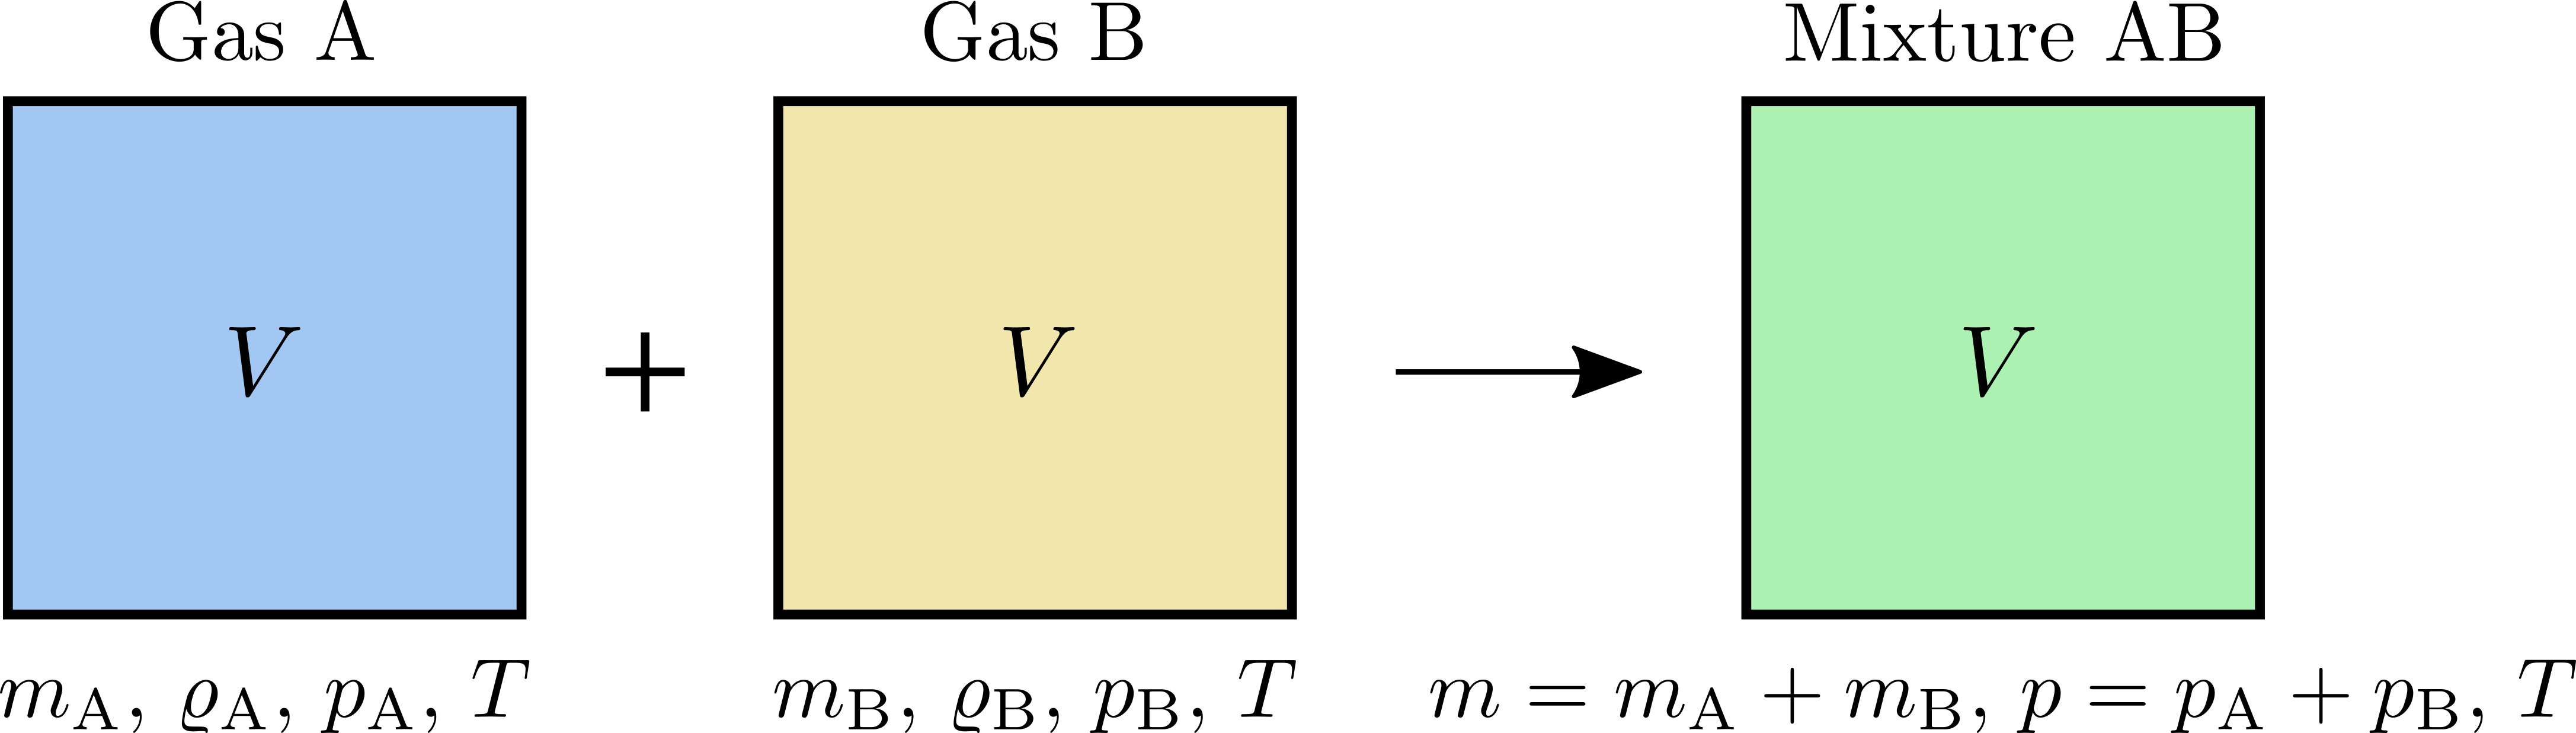
\includegraphics[width=0.7\textwidth]{png/dalton1.png}
  \caption{Dalton's law visualized}
  \label{fig:dalton1}
\end{figure}
%
The density of the mixture, $\varrho$, can be calculated as follows:
\begin{equation}
\varrho = \frac{m}{V} = \frac{m_\mathrm{A} + m_\mathrm{B}}{V} = \frac{\varrho_\mathrm{A} V + \varrho_\mathrm{B} V}{V} = \varrho_\mathrm{A} + \varrho_\mathrm{B},
\end{equation}
%
or for an arbitrary number of gases:
\begin{equation}
\varrho = \sum_{i}^{} \varrho_i ; \quad \varrho_m = \sum_{i}^{} \varrho_{m,i}.
\end{equation}
%
\subsubsection{Amagat's law}
Amagat's law assumes that the volumes of the component gases are additive; the interactions of the different gases are the same as the average interactions of the components. This is known as Amagat's law:
%
\begin{equation}
V = \sum_{i}^{}V_i.
\end{equation}
%
As an example, if two volumes of gas A and B at equal pressure are mixed, the pressure of the mixture stays the same, but the volumes add up (see Figure \ref{fig:dalton2}).
%
\begin{figure}[ht]
  \centering
  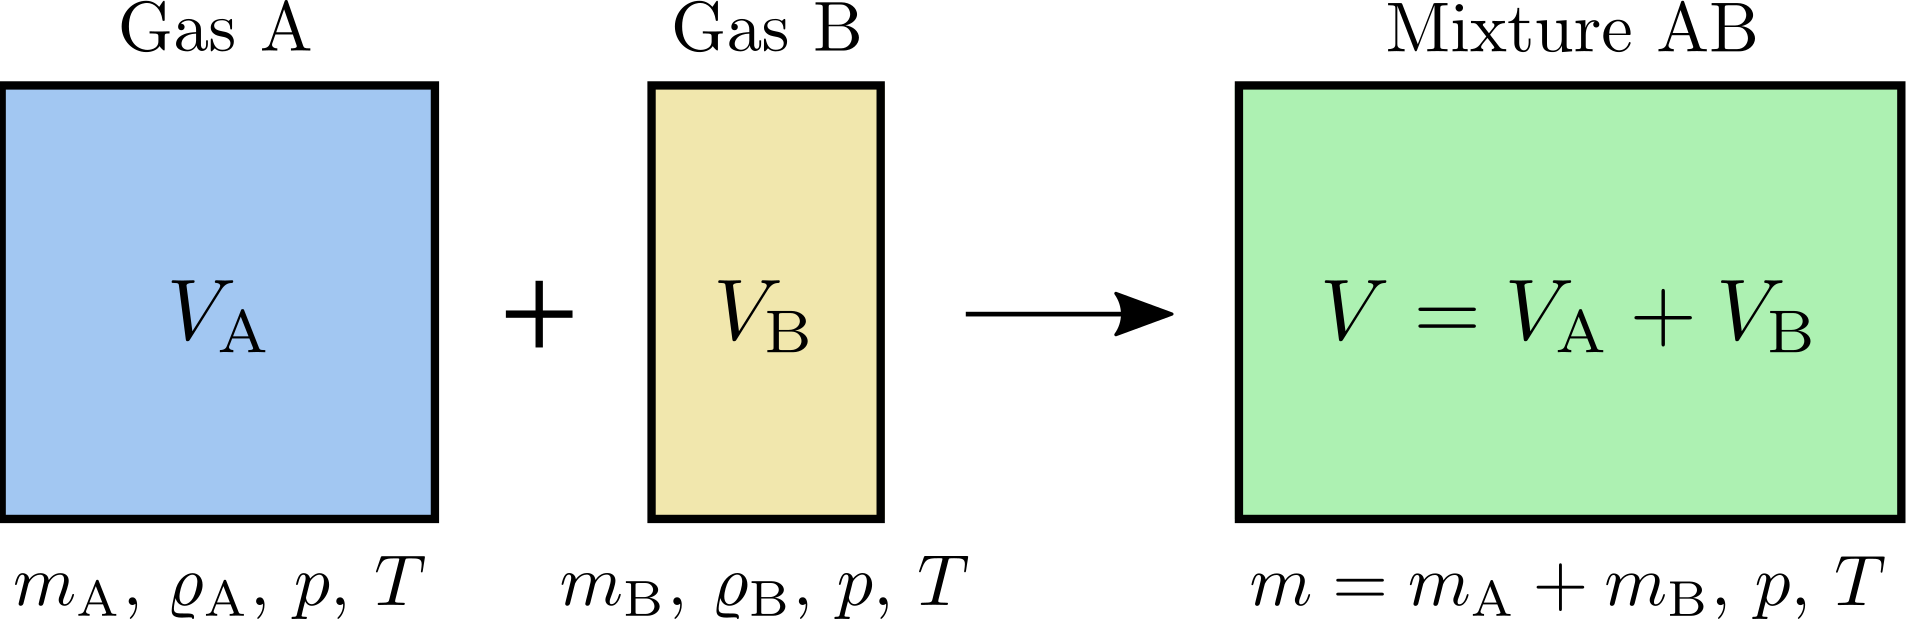
\includegraphics[width=0.7\textwidth]{png/dalton2.png}
  \caption{Amagat's law visualized}
  \label{fig:dalton2}
\end{figure}
%
The density of the mixture, $\varrho$, can be calculated as follows:
\begin{equation}
\varrho = \frac{m}{V} = \frac{m}{V_\mathrm{A} + V_\mathrm{B}} = \frac{m}{\frac{m_\mathrm{A}}{\varrho_\mathrm{A}} + \frac{m_\mathrm{B}}{\varrho_\mathrm{B}}} =
\frac{m}{\frac{X_\mathrm{A} m}{\varrho_\mathrm{A}} + \frac{X_\mathrm{B} m}{\varrho_\mathrm{B}}} = \frac{1}{\frac{X_\mathrm{A}}{\varrho_\mathrm{A}} + \frac{X_\mathrm{B}}{\varrho_\mathrm{B}}},
\end{equation}
%
or for an arbitrary number of gases:
%
\begin{equation}
\varrho = \frac{1}{\sum_{i}^{}\frac{X_i}{\varrho_i}}  ; \quad  \varrho_m = \frac{1}{\sum_{i}^{}\frac{x_i}{\varrho_{m,i}}}.
\end{equation}
%
\subsubsection{Ideal gases}
An ideal gas is defined as a gas whose molecules are spaced so far apart that the behavior of a molecule is not influenced by the presence of other molecules.
This assumption is usually valid at low pressures and high temperatures. The ideal gas law states that, for one gas:
%
\begin{equation}
p = \varrho \frac{RT}{M} ; \quad p= \varrho_m RT.
\end{equation}
%
Using the assumption of ideal gases and either Dalton's law or Amagat's law lead to the density of the mixture, $\varrho$, as:
%
\begin{equation}
\varrho = \frac{p}{RT} \sum_{i}^{}M_i x_i ; \quad \varrho_m = \frac{p}{RT}.
\end{equation}
%
\subsection{Available Models}
A list of all available models can be found
in the Doxygen documentation at
\url{https://dumux.org/docs/doxygen/releases/\DumuxVersion/modules.html}.
The documentation includes a detailed description for every model.

% SPDX-FileCopyrightInfo: Copyright © DuMux Project contributors, see AUTHORS.md in root folder
% SPDX-License-Identifier: CC-BY-4.0

\section{Temporal Discretization and Solution Strategies}
In this section, the temporal discretization as well as solution strategies (monolithic/sequential) are presented.

\subsection{Temporal discretization}

Our systems of partial differential equations are discretized in space and in time.

Let us consider the general case of a balance equation of the following form
\begin{equation}\label{eq:generalbalance}
\frac{\partial m(u)}{\partial t} + \nabla\cdot\mathbf{f}(u, \nabla u) + q(u) = 0,
\end{equation}
seeking an unknown quantity $u$ in terms of storage $m$, flux $\mathbf{f}$ and source $q$.
All available Dumux models can be written mathematically in form of \eqref{eq:generalbalance}
with possibly vector-valued quantities $u$, $m$, $q$ and a tensor-valued flux $\mathbf{f}$.
For the sake of simplicity, we assume scalar quantities $u$, $m$, $q$ and a vector-valued
flux $\mathbf{f}$ in the notation below.

For discretizing \eqref{eq:generalbalance}, we need to choose an
approximation for the temporal derivative $\partial m(u)/\partial t$.
While many elaborate methods for this approximation exist,
we focus on the simplest one of a first order difference quotient
\begin{equation}\label{eq:euler}
\frac{\partial m(u_{k/k+1})}{\partial t}
\approx \frac{m(u_{k+1}) - m(u_k)}{\Delta t_{k+1}}
\end{equation}
for approximating the solution $u$ at time $t_k$ (forward) or $t_{k+1}$ (backward).
The question of whether to choose the forward or the backward quotient leads to the
explicit and implicit Euler method, respectively.
In case of the former, inserting \eqref{eq:euler} in \eqref{eq:generalbalance}
at time $t_k$ leads to
\begin{equation}\label{eq:expliciteuler}
\frac{m(u_{k+1}) - m(u_k)}{\Delta t_{k+1}} + \nabla\cdot\mathbf{f}(u_k, \nabla u_k) + q(u_k) = 0,
\end{equation}
whereas the implicit Euler method is described as
\begin{equation}\label{eq:impliciteuler}
\frac{m(u_{k+1}) - m(u_k)}{\Delta t_{k+1}}
+ \nabla\cdot\mathbf{f}(u_{k+1}, \nabla u_{k+1}) + q(u_{k+1}) = 0.
\end{equation}
Once the solution $u_k$ at time $t_k$ is known, it is straightforward
to determine $m(u_{k+1})$ from \eqref{eq:expliciteuler},
while attempting to do the same based on \eqref{eq:impliciteuler}
involves the solution of a system of equations.
On the other hand, the explicit method \eqref{eq:expliciteuler} is stable only
if the time step size $\Delta t_{k+1}$ is below a certain limit that depends
on the specific balance equation, whereas the implicit method \eqref{eq:impliciteuler}
is unconditionally stable.

\subsection{Solution strategies to solve equations}
The governing equations of each model can be solved monolithically or sequentially.
The basic idea of the sequential algorithm is to reformulate the
equations of multi-phase flow into one equation for
pressure and equations for phase/component/... transport. The pressure equation
is the sum of the mass balance equations and thus considers the total flow of the
fluid system. The new set of equations is considered as decoupled (or weakly coupled)
and can thus be solved sequentially. The most popular sequential model is the
fractional flow formulation for two-phase flow which is usually implemented applying
an IMplicit Pressure Explicit Saturation algorithm (IMPES).
In comparison to solving the equations monolithically, the sequential structure allows the use of
different discretization methods for the different equations. The standard method
used in the sequential algorithm is a cell-centered finite volume method. Further schemes,
so far only available for the two-phase pressure equation, are cell-centered finite
volumes with multi-point flux approximation (Mpfa-O method) and mimetic finite differences.
An $h$-adaptive implementation of both sequential algorithms is provided for two dimensions.

\section{Spatial Discretization}
\label{spatialdiscretization}

We discretize space with cell-centered finite volume methods (\ref{cc} ), the box method (\ref{box})
or a staggered grid scheme (\ref{staggered}).
Grid adaption is available for both box and cell-centered finite volume method.
In general, the spatial  parameters, especially the porosity, have to be assigned on
the coarsest level of discretization.
%
\subsection{Cell Centered Finite Volume Methods -- A Short Introduction}\label{cc}
Cell-centered finite volume methods use the elements of the grid as control volumes.
For each control volume the discrete values are determined at the element/control
volume center (not required to be the barycenters).

We consider a domain $\Omega \subset \mathbb{R}^d$, $d \in \{ 2, 3 \}$ with boundary $\Gamma = \partial \Omega$. Within this section, we consider the following elliptic problem
\begin{equation}
  \begin{aligned}
                   \nabla \cdot \left( - \mathbf{\Lambda} \nabla u \right) &= q   &&\mathrm{in} \, \Omega \\
               \left( - \mathbf{\Lambda} \nabla u \right) \cdot \mathbf{n} &= v_N &&\mathrm{on} \, \Gamma_N \\
                                                                   u &= u_D &&\mathrm{on} \, \Gamma_D.
    \label{eq:elliptic}
  \end{aligned}
\end{equation}

Here, $\mathbf{\Lambda} = \mathbf{\Lambda}(\mathbf{x}, \mathbf{u})$ is a symmetric and positive definite tensor of second rank (e.g. permeability, diffusivity, etc.), $u = u (\mathbf{x})$ is unknown and $q = q(\mathbf{x}, \mathbf{u})$ is a source/sink.
We denote by $\mathcal{M}$ the mesh that results from the division of the domain $\Omega$ into $n_e$ control volumes $K \subset \Omega$. Each $K$ is a polygonal open set such that $K \cap L = \emptyset, \forall{K \neq L}$ and $\overline{\Omega} = \cup_{K \in \mathcal{M}} \overline{K}$.

For the derivation of the finite-volume formulation we integrate the first equation of \eqref{eq:elliptic} over a control volume $K$ and apply the Gauss divergence theorem:

\begin{equation}
    \int_{\partial K} \left( - \mathbf{\Lambda} \nabla u \right) \cdot \mathbf{n} \, \mathrm{d} \Gamma = \int_K q \, \mathrm{d}x.
    \label{eq:ellipticIntegrated}
\end{equation}

Splitting the control volume boundary $\partial K$ into a finite number of faces $\sigma \subset \partial K$ (such that $\sigma = \overline{K} \cap \overline{L}$ for some neighboring control volume $L$) and replacing the exact fluxes by an approximation, i.e. $F_{K, \sigma} \approx \int_{\sigma} \left( - \mathbf{\Lambda}_K \nabla u \right) \cdot \mathbf{n} \mathrm{d} \Gamma$ (here $\mathbf{\Lambda}_K$ is the value of $\mathbf{\Lambda}$ associated with control volume $K$), yield
\begin{equation}
    \sum_{\sigma \subset \partial K} F_{K, \sigma} = Q_K, \quad \forall \, {K \in \mathcal{M}},
\label{eq:ccdisc}
\end{equation}
where $F_{K, \sigma}$ is the discrete flux through face $\sigma$ flowing out of cell $K$ and $Q_K := \int_K q \, \mathrm{d}x$ is the integrated source/sink term. Equation \eqref{eq:ccdisc} is the typical cell-centered finite-volume formulation.
Finite-volume schemes differ in the way how the term
$(\mathbf{\Lambda}_K \nabla u ) \cdot \mathbf{n} $ is approximated (i.e. the choice of the fluxes $F_{K, \sigma}$). Using the symmetry of the tensor $\mathbf{\Lambda}_K$, this term can be rewritten as
$\nabla u  \cdot \mathbf{\Lambda}_K\mathbf{n}$, which corresponds to the directional derivative of $u$ in co-normal direction $\mathbf{\Lambda}_K\mathbf{n}$.
In the following, the main ideas of the two-point flux approximation and the multi-point flux approximation methods are briefly described. Hereby, we restrict the discussion to the two-dimensional case.

Please also note that other types of equations, e.g. instationary parabolic problems, can be discretized by applying some time discretization scheme to the time derivatives and by using the finite-volume scheme for the flux discretization. For simplicity the discussion is restricted to the elliptic problem \eqref{eq:elliptic}.

\subsubsection{Tpfa Method}\label{cc_tpfa}
The linear two-point flux approximation is a simple but robust cell-centered finite-volume scheme, which is commonly used in commercial software.
This scheme can be derived by using the co-normal decomposition, which reads
\begin{equation}
\mathbf{\Lambda}_K \mathbf{n}_{K, \sigma} = t_{K,\sigma} \mathbf{d}_{K,\sigma} + \mathbf{d}^{\bot}_{K,\sigma}, \quad  t_{K,\sigma} = \frac{\mathbf{n}_{K, \sigma}^T \mathbf{\Lambda}_K \mathbf{d}_{K,\sigma} }{\mathbf{d}_{K,\sigma}^T \mathbf{d}_{K,\sigma}}, \; \mathbf{d}^{\bot}_{K,\sigma} = \mathbf{\Lambda}_K \mathbf{n}_{K, \sigma} - t_{K,\sigma} \mathbf{d}_{K,\sigma},
\label{eq:conormalDecTpfa}
\end{equation}
with the tensor $\mathbf{\Lambda}_K$ associated with control volume $K$, the distance vector $\mathbf{d}_{K,\sigma} := \mathbf{x}_\sigma - \mathbf{x}_K$ and $\mathbf{d}_{K,\sigma}^T \mathbf{d}^{\bot}_{K,\sigma} = 0$, see Figure \ref{pc:cctpfa} for the used notations. The same can be done for the conormal $\mathbf{\Lambda}_L \mathbf{n}_{L, \sigma}$. The $t_{K,\sigma}$ and $t_{L,\sigma}$ are the transmissibilities associated with the face $\sigma$. These transmissibilities are calculated in \Dumux by using the function \texttt{computeTpfaTransmissibility}.

\begin{figure} [ht]
\centering

\includegraphics[width=0.4\linewidth,keepaspectratio]{png/cctpfa.png}
\caption{Two neighboring control volumes sharing the face $\sigma$.}
\label{pc:cctpfa}
\end{figure}


With these notations, it follows that for each cell $K$ and face $\sigma$
\begin{equation}
\nabla u \cdot \mathbf{\Lambda}_K \mathbf{n}_{K, \sigma} =  t_{K,\sigma} \nabla u \cdot \mathbf{d}_{K,\sigma} + \nabla u \cdot \mathbf{d}^{\bot}_{K,\sigma}.
\end{equation}
For the Tpfa scheme, the second part in the above equation is neglected. By using the fact that $\nabla u \cdot \mathbf{d}_{K,\sigma} \approx u_\sigma - u_K$, the discrete fluxes for face $\sigma$ are given by
\begin{equation}
F_{K,\sigma} = -\meas{\sigma}  t_{K,\sigma} (u_\sigma - u_K), \qquad F_{L,\sigma} = -\meas{\sigma}  t_{L,\sigma} (u_\sigma - u_L).
\label{eq:TPFAOneSided}
\end{equation}
Enforcing local flux conservation, i.e. $F_{K,\sigma}+F_{L,\sigma}=0$, results in
\begin{equation}
u_\sigma = \frac{t_{K,\sigma} u_K + t_{L,\sigma} u_L}{t_{K,\sigma}  + t_{L,\sigma}}.
\end{equation}
With this, the fluxes \eqref{eq:TPFAOneSided} are rewritten as
\begin{equation}
F_{K,\sigma} = \meas{\sigma}  \frac{t_{K,\sigma} t_{L,\sigma}}{t_{K,\sigma} + t_{L,\sigma}} (u_K - u_L), \quad F_{L,\sigma} = \meas{\sigma}  \frac{t_{K,\sigma} t_{L,\sigma}}{t_{K,\sigma} + t_{L,\sigma}} (u_L - u_K).
\label{eq:TPFAFlux}
\end{equation}
By neglecting the orthogonal term, the consistency of the scheme is lost for general grids, where $\nabla u \cdot \mathbf{d}^{\bot}_{K,\sigma} \not = 0$. The consistency is achieved only for so-called K-orthogonal grids for which $\mathbf{d}^{\bot}_{K,\sigma} = 0$. For such grids we deduce that
\begin{equation}
\frac{t_{K,\sigma} t_{L,\sigma}}{t_{K,\sigma} + t_{L,\sigma}} = \frac{\tau_{K,\sigma} \tau_{L,\sigma}}{\tau_{K,\sigma} d_{L,\sigma} + \tau_{L,\sigma} d_{K,\sigma}},
\label{eq:TPFAcoeffNew}
\end{equation}
with $\tau_{K,\sigma} := \mathbf{n}_{K, \sigma} \mathbf{\Lambda}_K\mathbf{n}_{K, \sigma}, \tau_{L,\sigma} := \mathbf{n}_{L, \sigma} \mathbf{\Lambda}_L\mathbf{n}_{L, \sigma}$, $d_{K,\sigma}:= \mathbf{n}_{K, \sigma} \cdot \mathbf{d}_{K, \sigma}$, and $d_{L,\sigma}:= \mathbf{n}_{L, \sigma} \cdot \mathbf{d}_{L, \sigma}$. This reduces, for the case of scalar permeability, to a distance weighted harmonic averaging of permeabilities.



\subsubsection{Mpfa Method}\label{cc_mpfa}
Expressions for the face fluxes $F_{K, \sigma}$ are obtained by introducing intermediate face unknowns $u_\sigma$ in addition to the cell unknowns $u_K$ and enforcing the physically motivated continuity of fluxes and continuity of the solution across the faces. For a face $\sigma$ between the two polygons $K$ and $L$ these conditions read:
\begin{equation}
    \begin{aligned}
        &F_{K, \sigma} + F_{L, \sigma} = 0 \\
        &{u}_{K,\sigma} = {u}_{L,\sigma} = {u}_{\sigma}.
        \label{eq:sigmaConditions}
    \end{aligned}
\end{equation}
Using these conditions, the intermediate face unknowns ${u}_\sigma$ can be eliminated and the fluxes are expressed as a function of the cell unknowns $u_N$ and associated transmissibilities $t^N_{K,\sigma}$:

\begin{equation}
    F_{K,\sigma} = \sum_{N \in \mathcal{S}_{K,\sigma}} t^N_{K,\sigma} u_{N}.
    \label{eq:FVFluxExpression}
\end{equation}

\begin{figure} [ht]
\centering
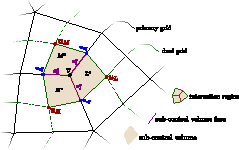
\includegraphics[width=0.8\linewidth,keepaspectratio]{pdf/mpfa_iv.pdf}
\caption{Interaction region for the Mpfa-O method. The graphic on the right illustrates how the sub-control volume $L^v$ and face $\sigma^v_2$ are embedded in cell $L$. Note that the face stencils for all sub-control volume faces in the depicted interaction region are $\mathcal{S}_{\sigma^v_i} = \{ K,L,M \}$, meaning that the fluxes over the sub-control volume faces depend on the three cell unknowns $u_K, u_L, u_M$.}
\label{pc:interactionRegion_mpfa}
\end{figure}

The main difference between the various finite-volume schemes available is the assembly of the face fluxes, i.e. the computation of the $t^N_{K,\sigma}$ and the size of $\mathcal{S}_{K,\sigma}$. For the Tpfa, that has been presented in the last section, the stencil and transmissibilities are given as
\begin{equation*}
\mathcal{S}_{K,\sigma} = \lbrace K,L \rbrace, \quad t^K_{K,\sigma} =  \meas{\sigma}  \frac{t_{K,\sigma} t_{L,\sigma}}{t_{K,\sigma} + t_{L,\sigma}},\; t^L_{K,\sigma} =  -\meas{\sigma}  \frac{t_{K,\sigma} t_{L,\sigma}}{t_{K,\sigma} + t_{L,\sigma}},
\end{equation*}
with $t_{K,\sigma},t_{L,\sigma}$ as defined in equation \eqref{eq:conormalDecTpfa}.

In the following, a multi-point flux approximation method (Mpfa-O method), which was introduced in \citet{A3:aavatsmark:2002}, is presented. The main difference to the Tpfa scheme is the fact that a consistent discrete gradient is constructed, i.e. the term $\nabla u \cdot \mathbf{d}^{\bot}_{K,\sigma}$ is not neglected.

For this scheme, a dual grid is created by connecting the barycenters of the cells with the barycenters of the faces ($d=2$) or the barycenters of the faces and edges ($d=3$). This divides each cell into sub-control volumes $K^v$. Analogously, each face is sub-divided into sub-control volume faces $\sigma^v$, see Figure \ref{pc:interactionRegion_mpfa}. We allow for piecewise constant $\mathbf{\Lambda}$ (denoted as $\mathbf{\Lambda}_K$ for each cell $K$) and construct discrete gradients $\nabla_\mathcal{D}^{K^v} u$ (per sub-control volume $K^v$).
In the following, we restrict our discussion to the two-dimensional setup that is shown in Figure \ref{pc:interactionRegion_mpfa}.
Here, the discrete gradients are constructed to be consistent such that the following conditions hold:
\begin{equation}
\nabla_\mathcal{D}^{K^v} u \cdot (\mathbf{x}_{\sigma^v_1}- \mathbf{x}_{K}) = u_{\sigma^v_1} - u_K, \quad \nabla_\mathcal{D}^{K^v} u \cdot (\mathbf{x}_{\sigma^v_3}- \mathbf{x}_{K}) = u_{\sigma^v_3} - u_K.
\end{equation}
Thus, a discrete gradient (for sub-control volume $K^v$) that fulfills  these conditions is given as
\begin{equation}
\nabla_\mathcal{D}^{K^v} u  = \mathbb{D}^{-T}_{K^v}
 \begin{bmatrix}
  u_{\sigma^v_1} - u_K \\
  u_{\sigma^v_3} - u_K
 \end{bmatrix}, \qquad \text{ with }\; \mathbb{D}_{K^v} :=
  \begin{bmatrix}
   \mathbf{x}_{\sigma^v_1}- \mathbf{x}_K & \mathbf{x}_{\sigma^v_3} - \mathbf{x}_K
 \end{bmatrix}.
 \label{eq:MPFAGradientRecons}
\end{equation}

This enables us to write the discrete flux across $\sigma^v_1$ from cell $K$ as follows:
\begin{equation}
    F_{K, \sigma^v_1} := - |\sigma^v_1| \mathbf{n}_{\sigma^v_1}^T \mathbf{\Lambda}_K \nabla_\mathcal{D}^{K^v} u.
    \label{eq:discreteFlux}
\end{equation}
Inserting the discrete gradient, yields
\begin{equation}
    F_{K, \sigma^v_1} = \omega_{K,\sigma^v_1\sigma^v_1}(u_K - u_{\sigma^v_1}) + \omega_{K,\sigma^v_1 \sigma^v_3}(u_K - u_{\sigma^v_3}),
    \label{eq:discreteFluxRef}
\end{equation}
with $(\omega_{K,\sigma^v_1\sigma^v_1},\omega_{K,\sigma^v_1 \sigma^v_3})^T = |\sigma^v_1| \mathbb{D}^{-1}_{K^v}\mathbf{\Lambda}_K \mathbf{n}_{\sigma^v_1}$. These values are calculated in \Dumux by using the function \texttt{computeMpfaTransmissibility}.
\\ \ \\
To deduce a cell-centered scheme, the introduced face unknowns $u_{\sigma^v_i}$ have to be eliminated. This is done by enforcing flux continuity for each sub-control volume face, i.e.
\begin{align}
F_{K, \sigma^v_1} + F_{L, \sigma^v_1} &= 0, \\ F_{K, \sigma^v_3} + F_{M, \sigma^v_3} &= 0, \\ F_{L, \sigma^v_2} + F_{M, \sigma^v_2} &= 0.
\end{align}
This results in a system of equations for the face unknowns $\mathbf{u}_{\sigma}$
\begin{equation}
\mathbb{A}^{3\times 3} \mathbf{u}_{\sigma} = \mathbb{B}^{3\times 3} \mathbf{u},
\end{equation}
where $\mathbf{u}$ contains the three cell unknowns $u_K,u_L,u_M$ and $\mathbf{u}_{\sigma}$ the three face unknowns $u_{\sigma^v_1}, u_{\sigma^v_2}, u_{\sigma^v_3}$.
Inserting these face unknowns into the flux expression \eqref{eq:discreteFluxRef} yields
\begin{equation}
    F_{K,\sigma^v_i} = \sum_{N \in \lbrace K,L,M \rbrace } t^N_{K,\sigma^v_i} u_{N} = \mathbf{t}_{K,\sigma^v_i} \cdot \mathbf{u},
    \label{eq:FVFluxExpressionSubFace}
\end{equation}
for each cell $K$ and sub-control volume face $\sigma^v_i$.
%
%
\subsection{Box Method -- A Short Introduction}\label{box}

The so called box method unites the advantages of the finite-volume (FV) and
finite-element (FE) methods.

First, the model domain $\Omega$ is discretized with a FE mesh consisting of nodes
$i$ and corresponding elements $E_k$. Then, a secondary FV mesh is constructed
by connecting the midpoints and barycenters of the elements surrounding node
$i$ creating a box $B_i$ around node $i$ (see Figure \ref{pc:box}a).

\begin{figure} [ht]
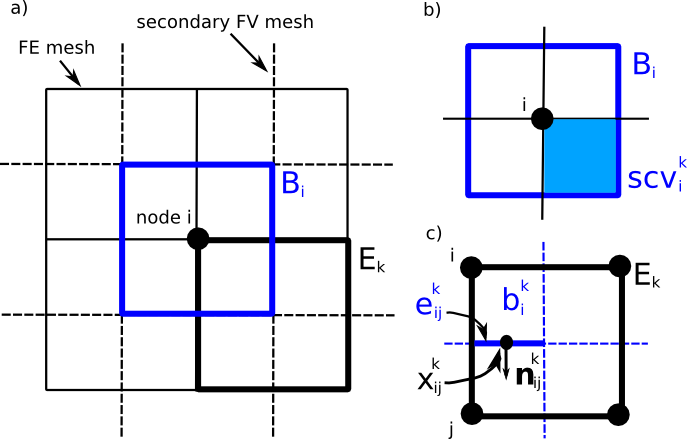
\includegraphics[width=0.8\linewidth,keepaspectratio]{png/box_disc.png}
\caption{\label{pc:box} Discretization of the box method}
\end{figure}

The FE mesh divides the box $B_i$ into subcontrolvolumes (scv's) $b^k_i$
(see Figure \ref{pc:box}b). Figure \ref{pc:box}c shows the finite element $E_k$
and the scv's $b^k_i$ inside $E_k$, which belong to four different boxes $B_i$.
Also necessary for the discretization are the faces of the subcontrolvolumes (scvf's)
$e^k_{ij}$ between the scv's $b^k_i$ and $b^k_j$, where $|e^k_{ij}|$ is the length
of the scvf. The integration points $x^k_{ij}$ on $e^k_{ij}$ and the outer normal
vector $\mathbf n^k_{ij}$ are also to be defined (see Figure \ref{pc:box}c).

The advantage of the FE method is that unstructured grids can be used, while the
FV method is mass conservative. The idea is to apply the FV method (balance of
fluxes across the interfaces) to each FV box $B_i$  and to get the fluxes across
the interfaces $e^k_{ij}$ at the integration points $x^k_{ij}$ from the FE approach.
Consequently, at each scvf the following expression results:

\begin{equation}
   f(\tilde u(x^k_{ij})) \cdot \mathbf n^k_{ij} \: |e^k_{ij}| \qquad \textrm{with}
   \qquad \tilde u(x^k_{ij}) = \sum_i N_i(x^k_{ij}) \cdot \hat u_i .
\end{equation}

In the following, the discretization of the balance equation is going to be derived.
From the \textsc{Reynolds} transport theorem follows the general balance equation:

\begin{equation}
  \underbrace{\int_\Omega \frac{\partial}{\partial t} \: u \, \mathrm{d}x}_{1}
  + \underbrace{\int_{\partial\Omega} (\mathbf{v} u + \mathbf w) \cdot \textbf n \, \mathrm{d}\Gamma}_{2} = \underbrace{\int_\Omega q \, \mathrm{d}x}_{3}
\end{equation}

\begin{equation}
  f(u) = \int_\Omega \frac{\partial u}{\partial t} \, \mathrm{d}x + \int_{\Omega} \nabla \cdot
  \underbrace{\left[  \mathbf{v} u + \mathbf w(u)\right] }_{F(u)}  \, \mathrm{d}x - \int_\Omega q \, \mathrm{d}x = 0
\end{equation}
where term 1 describes the changes of entity $u$ within a control volume over
time, term 2 the advective, diffusive and dispersive fluxes over the interfaces
of the control volume and term 3 is the source and sink term. $\Omega$ denotes the
model domain and $F(u) = F(\mathbf v, p) = F(\mathbf v(x,t), p(x,t))$.

Like the FE method, the box method follows the principle of weighted residuals.
In the function $f(u)$ the unknown $u$ is approximated by discrete values at the
nodes of the FE mesh $\hat u_i$ and linear basis functions $N_i$ yielding an
approximate function $f(\tilde u)$. For $u\in \lbrace \mathbf v, p, x^\kappa \rbrace$, this means:

\begin{minipage}[b]{0.47\textwidth}
\begin{equation}
\label{eq:p}
  \tilde p = \sum_i N_i \hat{p}_i
\end{equation}
\begin{equation}
\label{eq:v}
  \tilde{\mathbf v} = \sum_i N_i \hat{\mathbf v}_i
\end{equation}
\begin{equation}
\label{eq:x}
  \tilde x^\kappa  = \sum_i N_i \hat x_i^\kappa
\end{equation}
\end{minipage}
\hfill
\begin{minipage}[b]{0.47\textwidth}
\begin{equation}
\label{eq:dp}
  \nabla \tilde p = \sum_i \nabla N_i \hat{p}_i
\end{equation}
\begin{equation}
\label{eq:dv}
  \nabla \tilde{\mathbf v} = \sum_i \nabla N_i \hat{\mathbf v}_i
\end{equation}
\begin{equation}
\label{eq:dx}
  \nabla \tilde x^\kappa  = \sum_i \nabla N_i \hat x_i^\kappa .
\end{equation}
\end{minipage}

Due to the approximation with node values and basis functions, the differential equations are not exactly fulfilled anymore but a residual $\varepsilon$ is produced.

\begin{equation}
  f(u) = 0  \qquad \Rightarrow \qquad f(\tilde u) = \varepsilon
\end{equation}

Application of the principle of weighted residuals, meaning the multiplication
of the residual $\varepsilon$ with a weighting function $W_j$  and claiming that
this product has to vanish within the whole domain,

\begin{equation}
  \int_\Omega \varepsilon W_j \, \mathrm{d}x \overset {!}{=} \: 0 \qquad \textrm{with} \qquad \sum_j W_j =1
\end{equation}
yields the following equation:

\begin{equation}
  \int_\Omega \frac{\partial \tilde u}{\partial t} W_j \, \mathrm{d}x + \int_\Omega
   \left[ \nabla \cdot F(\tilde u) \right] W_j  \, \mathrm{d}x - \int_\Omega q W_j \, \mathrm{d}x = \int_\Omega \varepsilon W_j \, \mathrm{d}x \: \overset {!}{=} \: 0.
\label{eq:weightedResidual}
\end{equation}

For standard Galerkin schemes, the weighting functions $W_j$ are chosen the same as the ansatz functions $N_j$. However, this does not yield a locally mass-conservative scheme.
Therefore, for the Box method, the weighting functions $W_j$ are chosen as
the piece-wise constant functions over a
control volume box $B_j$, i.e.

\begin{equation}
  W_j(x) = \begin{cases}
            1 &x \in B_j \\
      0 &x \notin B_j.\\
           \end{cases}
\label{eq:weightingFunctions}
\end{equation}
Thus, the Box method is a Petrov-Galerkin scheme, where the weighting functions do not belong to the same function space than the ansatz functions.

Inserting definition \eqref{eq:weightingFunctions} into equation \eqref{eq:weightedResidual} and using the \textsc{Green-Gaussian} integral theorem results in
\begin{equation}
  \int_{B_j} \frac{\partial \tilde u}{\partial t} \, \mathrm{d}x + \int_{\partial B_j}  F(\tilde u) \cdot \mathbf n \, \mathrm{d}\Gamma_{B_j} - \int_{B_j} q \, \mathrm{d}x  \overset {!}{=} \: 0,
\label{eq:BoxMassBlance}
\end{equation}
which has to hold for every box $B_j$.

The first term in equation \eqref{eq:BoxMassBlance} can be written as
\begin{equation}
\int_{B_j} \frac{\partial \tilde u}{\partial t} \, \mathrm{d}x = \frac{d}{dt} \int_{B_j} \sum_i \hat u_i N_i  \, \mathrm{d}x = \sum_i \frac{\partial \hat u_i}{\partial t} \int_{B_j}  N_i  \, \mathrm{d}x.
\end{equation}
Here, a mass lumping technique is applied by assuming that the storage capacity is
reduced to the nodes. This means that the integrals $M_{i,j} = \int_{B_j}  N_i \, \mathrm{d}x$
are replaced by some mass lumped terms $M^{lump}_{i,j}$ which are defined as
\begin{equation}
   M^{lump}_{i,j} =\begin{cases}  |B_j| &j = i\\
  0 &j \neq i,\\
           \end{cases}
\end{equation}
where $|B_j|$ is the volume of the FV box $B_j$ associated with node $j$.
The application of this assumption yields

\begin{equation}
\label{eq:disc1}
  |B_j| \frac{\partial \hat u_j}{\partial t}
  +  \int_{\partial B_j}  F(\tilde u) \cdot \mathbf n \, \mathrm{d}\Gamma_{B_j} - Q_j = 0,
\end{equation}
where $Q_j$ is an approximation (using some quadrature rule) of the integrated source/sink term $\int_{B_j} q \, \mathrm{d}x$.

Using an implicit Euler time discretization finally
leads to the discretized form which will be applied to the mathematical
flow and transport equations:

\begin{equation}
\label{eq:discfin}
  |B_j| \frac{\hat u_j^{n+1} - \hat u_j^{n}}{\Delta t}
  + \int_{\partial B_j}  F(\tilde u^{n+1}) \cdot \mathbf n
  \;   \mathrm{d}\Gamma_{B_j} - Q_j^{n+1} \: = 0.
\end{equation}
Equation \eqref{eq:discfin} has to be fulfilled for each box $B_j$.
%
\subsection{Staggered Grid -- A Short Introduction}\label{staggered}

\begin{figure}[ht]
\centering
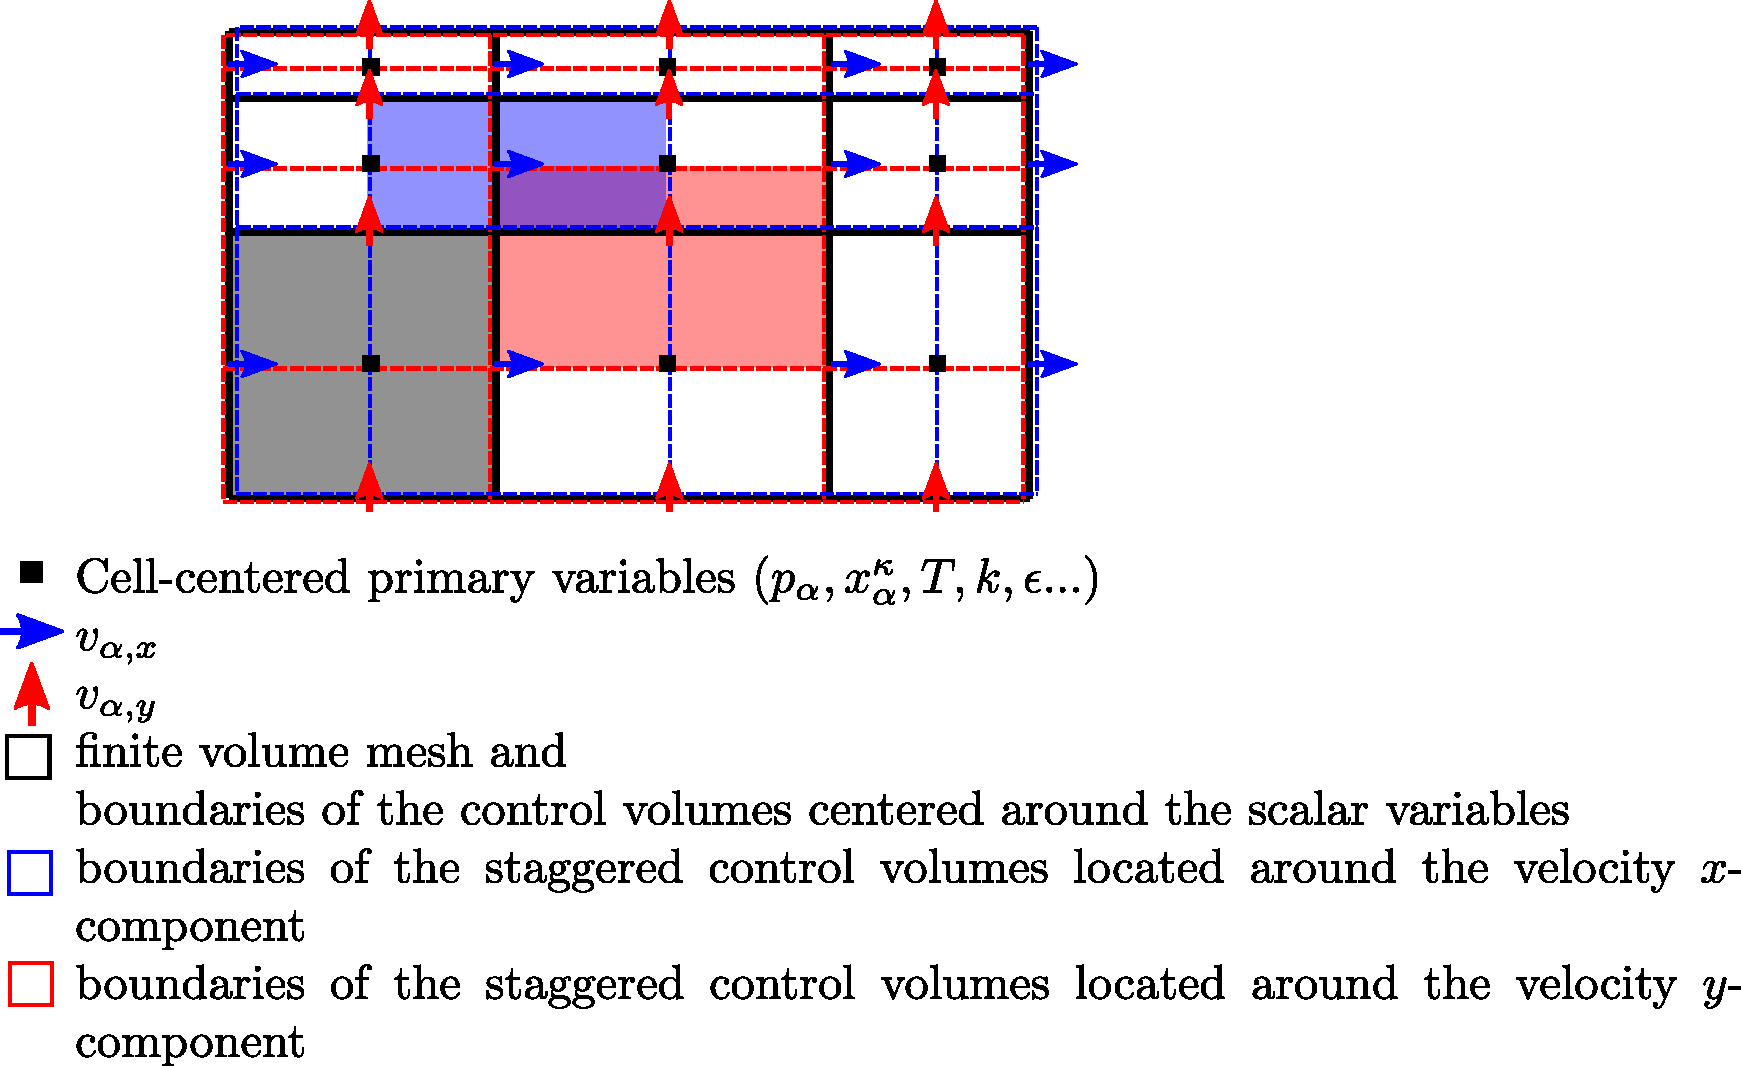
\includegraphics[width=.8\linewidth]{./pdf/staggered_grid.pdf}
\caption{\label{pc:staggered} Discretization of the staggered-grid method. The figure shows the different control volume arrangements, which are staggered with respect to each other. There are the control volumes centered around the scalar primary variables in black, the control volumes located around the $x$-component of the velocity in blue and the control volumes located around the $y$-components of the velocity in red. The control volume boundaries are given by lines. Additionally, there is one shaded example control volume each.\\
In the two-dimensional free-flow models, the continuity equation is discretized using the black control volumes, the $x$-component of the momentum equation is discretized using the blue control volumes and the $y$-component is discretized using the red control volumes. In three dimensions this works analogously.}
\end{figure}

The staggered-grid or marker-and-cell method uses a finite volume method with different control volumes for different equations. There are control volumes centered around the scalar primary variables. They correspond to the finite volume mesh. Additionally, there are control volumes located around the $x,y$ and (in 3D) $z$ velocity components which are shifted in the $x,y$ and $z$ direction, such that the velocity components are located on the edges of the cell-centered finite volume mesh (see Figure~\ref{pc:staggered}). As for the cell-centered method, the fluxes are evaluated at the edges of each control volume with a two-point flux approximation, cf. \ref{cc}.\par
The staggered-grid method is robust, mass conservative, and free of pressure oscillations
but should, as the cell-centered TPFA method, only be applied for structured grids.
Currently, all free-flow models in \Dumux use the staggered-grid discretization.

\section{Steps of a \Dumux Simulation}
\label{flow}


This chapter is supposed to give a short overview over how things are ``handed around'' in \Dumux. It
is not a comprehenisve guide through the modeling framework of \Dumux, but
hopefully it will help getting to grips with it.

In Section \ref{content} the structure of \Dumux is shown from a \emph{content}
point of view.

\subsection{Structure -- by Content}

\label{content}
In Figure \ref{fig:algorithm}, the algorithmic representations of a monolithical
solution scheme is illustrated down to the element level.

\begin{figure}[hbt]
\setcounter{thingCounter}{0}

\scriptsize
\sffamily
\begin{center}\parbox{0cm}{
\begin{tabbing}
\textbf{{\begin{turn}{45}\color{black}\numberThis{main}{init}\end{turn}}}             \=
\textbf{{\begin{turn}{45}\color{dumuxBlue}\numberThis{time step}{prep}\end{turn}}}            \=
\textbf{{\begin{turn}{45}\color{Mulberry}\numberThis{\textsc{Newton}}{elem}\end{turn}}}         \=
\textbf{{\begin{turn}{45}\color{dumuxYellow}\numberThis{element}{calc}\end{turn}}}             \=  \\
\\
\color{black}initialize \\
\color{black}\textbf{foreach} time step\\

  \> \color{dumuxBlue}\textbf{foreach} \textsc{Newton} iteration \\

    \> \> \color{Mulberry}\textbf{foreach} element \\

      \> \> \> \color{dumuxYellow}- calculate element \\
      \> \> \> \color{dumuxYellow}\; residual vector and \\
      \> \> \> \color{dumuxYellow}\; Jacobian matrix\\
      \> \> \> \color{dumuxYellow}- assemble into global\\
      \> \> \> \color{dumuxYellow}\; residual vector and \\
      \> \> \> \color{dumuxYellow}\;{Jacobian} matrix \\

    \> \> \color{Mulberry}\textbf{endfor} \\

    \> \> \color{Mulberry}solve linear system\\
    \> \> \color{Mulberry}update solution\\
    \> \> \color{Mulberry}check for \textsc{Newton} convergence\\
  \> \color{dumuxBlue}\textbf{endfor}\\
  \> \color{dumuxBlue}- adapt time step size, \\
  \> \color{dumuxBlue}\; possibly redo with smaller step size\\
  \> \color{dumuxBlue}- write result\\
\color{black}\textbf{endfor}\\
\color{black}finalize
\end{tabbing}}
\end{center}
\caption{Structure of a monolithical solution scheme in \Dumux.}
\label{fig:algorithm}
\end{figure}

\subsection{Structure -- by Implementation}
A possible starting point to understand how the above mentioned algorithm is implemented within \Dumux,
is the example main file
\url{https://git.iws.uni-stuttgart.de/dumux-repositories/dumux-course/releases/3.0/exercises/exercise-mainfile/exercise_1p_a.cc}

\section{Property System}
\label{sec:propertysystem}
A high level overview over the property system's design and principle ideas
are given, then follows a reference and a self-contained example.

\subsection{Motivation and features}
The \Dumux property system is a traits system
which allows easy inheritance.
In the context of the \Dumux property system, a property is an arbitrary
class body which may contain type definitions, values and methods.
Just like normal classes, properties can be arranged in hierarchies. In
the context of the \Dumux property system, nodes of the inheritance
hierarchy are called \emph{type tags}.

It also supports \emph{property nesting}. Property nesting means that the definition of
a property can depend on the value of other properties which may be
defined for arbitrary levels of the inheritance hierarchy.

\subsection{How-to}
All source files which use the property system should include
the header file \path{dumux/common/properties/propertysystem.hh}.
Declaration of type tags and
property tags as well as defining properties must be done inside the
namespace \texttt{Dumux::Properties}.

\subsubsection{Defining Type Tags}
New nodes in the type tag hierarchy can be defined in the \texttt{TTag} namespace using
\begin{lstlisting}[style=DumuxCode]
// Create new type tags
namespace TTag {
struct NewTypeTagName { using InheritsFrom = std::tuple<BaseTagName1, BaseTagName2, ...>; };
} // end namespace TTag
\end{lstlisting}
where the \texttt{InheritsFrom} alias is optional. To avoid
inconsistencies in the hierarchy, each type tag may be defined only
once for a program. If you call \texttt{GetProp} the property system will first look for the properties defined in \texttt{BaseTagName1} in the \texttt{InheritsFrom} list.
If a defined property is found this property is returned. If no defined property is found the search will continue in the ancestors of \texttt{BaseTagName1}.
If again no defined property is found the search will continue in the second \texttt{BaseTagName2} in the list, and so on.
If no defined property is found at all, a compiler error is triggered.

\vskip1ex\noindent
Example:
\begin{lstlisting}[style=DumuxCode]
namespace Dumux {
namespace Properties {
namespace TTag {
struct MyBaseTypeTag1 {};
struct MyBaseTypeTag2 {};

struct MyDerivedTypeTag { using InheritsFrom = std::tuple<MyBaseTypeTag1, MyBaseTypeTag2>; };
} // end namespace TTag
}}
\end{lstlisting}

\subsubsection{Defining new Property Tags}
New property tags are defined using

\begin{lstlisting}[style=DumuxCode]
template<class TypeTag, class MyTypeTag>
struct NewPropTagName { using type = UndefinedProperty; };
\end{lstlisting}

\vskip1ex\noindent
Example:
\begin{lstlisting}[style=DumuxCode]
namespace Dumux {
namespace Properties {
template<class TypeTag, class MyTypeTag>
struct MyPropertyTag { using type = UndefinedProperty; };
}}
\end{lstlisting}

If you need to forward declare a property use

\begin{lstlisting}[style=DumuxCode]
// forward declaration
template<class TypeTag, class MyTypeTag>
struct NewPropTagName;
\end{lstlisting}

\subsubsection{Defining Properties}
The value of a property on a given node of the type tag hierarchy is
defined using
\begin{lstlisting}[style=DumuxCode]
template<class TypeTag>
struct PropertyTagName<TypeTag, TTag::TypeTagName>
{
  // arbitrary body of a struct
};
\end{lstlisting}

This means a property is defined for a specific type tag node \texttt{TTag::TypeTagName}
by providing a partial template specialization of \texttt{PropertyTagName}.
The body typically contains either the alias \texttt{type}, or a data member \texttt{value}.
However, you can of course write in the body whatever you like.

\begin{lstlisting}[style=DumuxCode]
template<class TypeTag>
struct PropertyTagName<TypeTag, TTag::TypeTagName> { using type = type; };

template<class TypeTag>
struct PropertyTagName<TypeTag, TTag::TypeTagName> { static constexpr bool value = booleanValue; };

template<class TypeTag>
struct PropertyTagName<TypeTag, TTag::TypeTagName> { static constexpr int value = integerValue; };
\end{lstlisting}

\vskip1ex\noindent
Example:
\begin{lstlisting}[style=DumuxCode]
namespace Dumux {
namespace Properties {

// Create new type tag
namespace TTag {
struct MyTypeTag {};
}

// Define some properties
template<class TypeTag, class MyTypeTag> struct MyCustomProperty { using type = UndefinedProperty; };
template<class TypeTag, class MyTypeTag> struct MyType { using type = UndefinedProperty; };
template<class TypeTag, class MyTypeTag> struct MyBoolValue { using type = UndefinedProperty; };
template<class TypeTag, class MyTypeTag> struct MyIntValue { using type = UndefinedProperty; };
template<class TypeTag, class MyTypeTag> struct MyScalarValue { using type = UndefinedProperty; };

// Set the properties for the new type tag
template<class TypeTag>
struct MyCustomProperty<TypeTag, TTag::MyTypeTag>
{
    static void print()
    { std::cout << "Hello, World!\n"; }
};

template<class TypeTag>
struct MyType<TypeTag, TTag::MyTypeTag> { using type = unsigned int; };

template<class TypeTag>
struct MyBoolValue<TypeTag, TTag::MyTypeTag> { static constexpr bool value = true; };

template<class TypeTag>
struct MyIntValue<TypeTag, TTag::MyTypeTag> { static constexpr int value = 12345; };

template<class TypeTag>
struct MyScalarValue<TypeTag, TTag::MyTypeTag> { static constexpr double value = 12345.67890; };
}}
\end{lstlisting}

\subsubsection{Retrieving Property Values}
The type of a property can be retrieved using
\begin{lstlisting}[style=DumuxCode]
using Prop = GetProp<TypeTag, Properties::PropertyTag>;
\end{lstlisting}

There is a helper struct and a helper function to retrieve the \texttt{type} and \texttt{value}
members of a property

\begin{lstlisting}[style=DumuxCode]
using PropType = GetPropType<TypeTag, Properties::PropertyTag>;
constexpr auto propValue = getPropValue<TypeTag, Properties::PropertyTag>();
\end{lstlisting}

\vskip1ex\noindent
Example:\nolinebreak
\begin{lstlisting}[style=DumuxCode]
template <TypeTag>
class MyClass {
    // retrieve the ::value attribute of the 'UseMoles' property
    static constexpr bool useMoles = getPropValue<TypeTag, Properties::UseMoles>();
    static constexpr bool useMoles2 = GetProp<TypeTag, Properties::UseMoles>::value; // equivalent

    // retrieve the ::type attribute of the 'Scalar' property
    using Scalar = GetPropType<TypeTag, Properties::Scalar>;
    using Scalar2 = GetProp<TypeTag, Properties::Scalar>::type; // equivalent
};
\end{lstlisting}

\subsubsection{Nesting Property Definitions}
Inside property definitions there is access to all other properties
which are defined somewhere on the type tag hierarchy. The node for
which the current property is requested is available via the template argument
\texttt{TypeTag}. Inside property class bodies \texttt{GetPropType} can be used to
retrieve other properties and create aliases.

\vskip1ex\noindent
Example:
\begin{lstlisting}[style=DumuxCode]
template<class TypeTag>
struct Vector<TypeTag, TTag::MyModelTypeTag>
{
    using Scalar = GetPropType<TypeTag, Properties::Scalar>;
    using type = std::vector<Scalar>;
};
\end{lstlisting}

\subsection{A Self-Contained Example}
As a concrete example, let us consider some kinds of cars: Compact
cars, sedans, trucks, pickups, military tanks and the Hummer-H1 sports
utility vehicle. Since all these cars share some characteristics, it
makes sense to inherit those from the closest matching car type and
only specify the properties which are different. Thus, an inheritance
diagram for the car types above might look like outlined in Figure
\ref{fig:car-hierarchy}.

\begin{figure}[t]
  \centering
  \subfloat[]{
    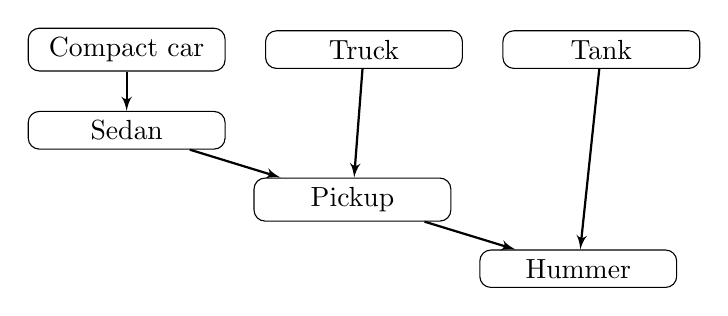
\begin{tikzpicture}
      [cars/.style={rectangle,draw=black,rounded corners,minimum width=2.5cm,node distance=0.5cm}]
      % place nodes
      \node[cars] (compact) {Compact car};
      \node[cars] (sedan) [below=of compact] {Sedan};
      \node[cars] (truck) [right=of compact] {Truck};
      \node[cars] (pickup) [below right= of sedan] {Pickup};
      \node[cars] (tank) [right=of truck] {Tank};
      \node[cars] (hummer) [below right= of pickup] {Hummer};
      % add edges
      \draw [-latex',thick] (compact) -- (sedan);
      \draw [-latex',thick] (sedan) -- (pickup);
      \draw [-latex',thick] (truck) -- (pickup);
      \draw [-latex',thick] (tank) -- (hummer);
      \draw [-latex',thick] (pickup) -- (hummer);
    \end{tikzpicture}
    \label{fig:car-hierarchy}
  }
  \hspace*{0.5cm}
  \subfloat[]{
    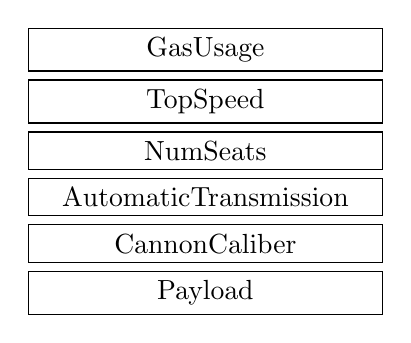
\begin{tikzpicture}
      [propertyBox/.style={rectangle,draw=black,minimum width=4.5cm,node distance=0.1cm}]
      \node[propertyBox] (gasUsage) {GasUsage};
      \node[propertyBox] (speed) [below=of gasUsage] {TopSpeed};
      \node[propertyBox] (seats) [below=of speed] {NumSeats};
      \node[propertyBox] (automatic) [below=of seats] {AutomaticTransmission};
      \node[propertyBox] (caliber) [below=of automatic] {CannonCaliber};
      \node[propertyBox] (payload) [below=of caliber] {Payload};
    \end{tikzpicture}
    \label{fig:car-propertynames}
  }
  \caption{\textbf{(a)}~A possible property inheritance graph for
    various kinds of cars.  The lower nodes inherit from higher ones;
    Inherited properties from nodes on the right take precedence over the
    properties defined on the left. \textbf{(b)}~Property names
    which make sense for at least one of the car types of (a).}
\end{figure}

Using the \Dumux property system, this inheritance hierarchy is
defined by:
\begin{lstlisting}[name=propsyscars,style=DumuxCode]
#include <dumux/common/propertysystem.hh>
#include <iostream>

namespace Dumux {
namespace Properties {
namespace TTag{
struct CompactCar {};
struct Truck {};
struct Tank {};

struct Sedan { using InheritsFrom = std::tuple<CompactCar>; };
struct Pickup { using InheritsFrom = std::tuple<Truck, Sedan>; };
struct HummerH1 { using InheritsFrom = std::tuple<Tank, Pickup>; };
}}} // end namespace TTag
\end{lstlisting}

Figure \ref{fig:car-propertynames} lists a few property names which
make sense for at least one of the nodes of Figure
\ref{fig:car-hierarchy}. These property names can be defined as
follows:
\begin{lstlisting}[name=propsyscars,style=DumuxCode]
template<class TypeTag, class MyTypeTag>
struct GasUsage { using type = UndefinedProperty; }; // [l/100km]
template<class TypeTag, class MyTypeTag>
struct TopSpeed { using type = UndefinedProperty; }; // [km/h]
template<class TypeTag, class MyTypeTag>
struct NumSeats { using type = UndefinedProperty; }; // []
template<class TypeTag, class MyTypeTag>
struct AutomaticTransmission { using type = UndefinedProperty; }; // true/false
template<class TypeTag, class MyTypeTag>
struct CannonCaliber { using type = UndefinedProperty; }; // [mm]
template<class TypeTag, class MyTypeTag>
struct Payload { using type = UndefinedProperty; }; // [t]
\end{lstlisting}

\noindent
So far, the inheritance hierarchy and the property names are completely
separate. What is missing is setting some values for the property
names on specific nodes of the inheritance hierarchy. Let us assume
the following:
\begin{itemize}
\item For a compact car, the top speed is the gas usage in $\unitfrac{l}{100km}$
  times $30$, the number of seats is $5$ and the gas usage is
  $\unitfrac[4]{l}{100km}$.
\item A truck is by law limited to $\unitfrac[100]{km}{h}$ top speed, the number
  of seats is $2$, it uses $\unitfrac[18]{l}{100km}$ and has a cargo payload of
  $\unit[35]{t}$.
\item A tank exhibits a top speed of $\unitfrac[60]{km}{h}$, uses $\unitfrac[65]{l}{100km}$
  and features a $\unit[120]{mm}$ diameter cannon
\item A sedan has a gas usage of $\unitfrac[7]{l}{100km}$, as well as an automatic
  transmission, in every other aspect it is like a compact car.
\item A pick-up truck has a top speed of $\unitfrac[120]{km}{h}$ and a payload of
  $\unit[5]{t}$. In every other aspect it is like a sedan or a truck but if in
  doubt, it is more like a truck.
\item The Hummer-H1 SUV exhibits the same top speed as a pick-up
  truck.  In all other aspects it is similar to a pickup and a tank,
  but, if in doubt, more like a tank.
\end{itemize}

\noindent
Using the \Dumux property system, these assumptions are formulated
using
\begin{lstlisting}[name=propsyscars,style=DumuxCode]
template<class TypeTag>
struct TopSpeed<TypeTag, TTag::CompactCar>
{static constexpr int value = getPropValue<TypeTag, Properties::GasUsage>() * 30};

template<class TypeTag>
struct NumSeats<TypeTag, TTag::CompactCar> { static constexpr int value = 5; };

template<class TypeTag>
struct GasUsage<TypeTag, TTag::CompactCar> { static constexpr int value = 4; };

template<class TypeTag>
struct TopSpeed<TypeTag, TTag::Truck> { static constexpr int value = 100; };

template<class TypeTag>
struct NumSeats<TypeTag, TTag::Truck> { static constexpr int value = 2; };

template<class TypeTag>
struct GasUsage<TypeTag, TTag::Truck> { static constexpr int value = 18; };

template<class TypeTag>
struct Payload<TypeTag, TTag::Truck> { static constexpr int value = 35; };

template<class TypeTag>
struct TopSpeed<TypeTag, TTag::Tank> { static constexpr int value = 60; };

template<class TypeTag>
struct GasUsage<TypeTag, TTag::Tank> { static constexpr int value = 65; };

template<class TypeTag>
struct CannonCaliber<TypeTag, TTag::Tank> { static constexpr int value = 120; };

template<class TypeTag>
struct GasUsage<TypeTag, TTag::Sedan> { static constexpr int value = 7; };

template<class TypeTag>
struct AutomaticTransmission<TypeTag, TTag::Sedan> { static constexpr bool value = true; };

template<class TypeTag>
struct TopSpeed<TypeTag, TTag::Pickup> { static constexpr int value = 120; };

template<class TypeTag>
struct Payload<TypeTag, TTag::Pickup> { static constexpr int value = 5; };

template<class TypeTag>
struct TopSpeed<TypeTag, TTag::HummerH1>
{ static constexpr int value = getPropValue<TypeTag, TTag::Pickup::TopSpeed<TypeTag>>(); };
\end{lstlisting}

\noindent
Now property values can be retrieved and some diagnostic messages can
be generated. For example
\begin{lstlisting}[name=propsyscars,style=DumuxCode]
int main()
{
    std::cout << "top speed of sedan: " << getPropValue<Properties::TTag::Sedan, Properties::TopSpeed>() << "\n";
    std::cout << "top speed of truck: " << getPropValue<Properties::TTag::Truck, Properties::TopSpeed>() << "\n";
}
\end{lstlisting}
will yield the following output:
\begin{lstlisting}[style=Bash, basicstyle=\ttfamily\scriptsize\let\textcolor\textcolordummy]
$ top speed of sedan: 210
$ top speed of truck: 100
\end{lstlisting}

\section{Input and Output}
\label{sec:inputandoutput}

This section briefly explains grid generation in \Dumux, summarizes
the grid formats that can be used by \Dumux and introduces the \Dumux \texttt{GridManager}.
Finally, this section informs about handling output in \Dumux.

\subsection{Supported grid file formats}
\label{sec:supportedGridFormats}
\Dumux can read grids from file using the Dune Grid Format (DGF), the Gmsh mesh format (MSH), the Eclipse grid format (GRDECL), or the Visualization ToolKit (VTK/VTU/VTP) format. 

\subsubsection{Dune Grid Format}
Most of our \Dumux tests use the Dune Grid Format (DGF) to read in grids. A detailed description
of the DGF format and some examples can be found in the \Dune doxygen documentation
\textbf{(Modules $\rightarrow$ I/O $\rightarrow$ Dune Grid Format (DGF)}). To generate larger or more
complex DGF files, we recommend to write your own scripts, e.g, in \Cplusplus, Matlab or Python.

The DGF format can also be used to read in spatial parameters defined on the grid. These parameters can
be defined on nodes as well as on the elements. An example for predefined parameters on a grid
can be found in \texttt{dumux/test/porousmediumflow/co2/implicit/}.

\subsubsection{Gmsh Mesh Format}
Gmsh is an open-source flexible grid generator for unstructured finite-element meshes (\cite{GEUZAINE2009}, \url{http://geuz.org/gmsh/}).
\Dumux supports the default Gmsh mesh format (MSH). For the format specifics and how to create grids with Gmsh, e.g., using
the provided GUI, we refer to the Gmsh documentation (\url{http://geuz.org/gmsh/doc/texinfo/gmsh.html}).

The MSH format can contain element and boundary markers defined on the grid. Thus, boundaries can be easily marked as, e.g., inflow boundaries
using Gmsh. Further, the format supports higher order elements. They can be used to create boundary parametrization supported by, e.g., the grid
manager \texttt{UGGrid}.
An example can be found in \texttt{dumux/test\allowbreak/io/gridmanager}.

\subsubsection{Eclipse Grid Format}
The Eclipse Grid Format (GRDECL) is commonly used for corner-point grids.
Such grids consist of hexahedra, which are described by eight points on so-called pillars. A special feature of corner-point geometries is that points on pillars can degenerate, meaning that two neighboring points on a pillar can coincide. Furthermore, faces are, in general, bi-linear and cells can be non-convex. This allows for the accurate description of faults, layers, or wells, occurring in geological environments.

Furthermore, petrophysical properties can be defined (for each cell), by using eclipse-specific keywords, e.g. \texttt{PORO}, \texttt{PERMX}, \texttt{PERMY}.

\Dumux supports the Eclipse Grid Format by using the \texttt{opm-grid} module (see (\url{https://opm-project.org}).
An example can be found in \texttt{dumux/test\allowbreak/porousmediumflow/2p/implicit/cornerpoint}.

\subsubsection{VTK file format}


\subsubsection{Other Grid Formats}
Grid formats other than DGF, MSH, GRDECL, or VTK will have to be converted to the DGF, MSH, GRDECL, or VTK format before they can be used in \Dumux.
If conversion is not an option, another possibility would be to write your own \texttt{GridManager}s. Examples of other grid formats,
which have previously been either converted or custom-created in \Dumux, are ArtMesh grids (fractured network grids), and ICEM grids (CAD developed grids).

\subsection{The \Dumux \texttt{GridManager}}
The \texttt{Dumux::GridManager} class constructs the grid from information in the input file and handles the data.
Currently, supported Dune grid interface implementations  are \texttt{YaspGrid}, \texttt{OneDGrid}, \texttt{dune-uggrid}, \texttt{dune-alugrid}, \texttt{dune-foamgrid}, \texttt{dune-subgrid}, \texttt{opm-grid} (cornerpoint grids) and \texttt{dune-spgrid}.
Grids can be constructed from a DGF, VTK or MSH file by simply providing the filename to the grid in the \texttt{Grid} group~\footnote{Note,
that group name \texttt{Grid} is the default group name and can be customized in your problem changing the string property \texttt{GridParameterGroup}.
This way, it is possible, e.g., for problems with more than one grid, to set different group names for each grid, thus configuring them separately.}
of the input file:
\begin{lstlisting}[style=DumuxParameterFile]
[Grid]
File = mydgfgrid.dgf
\end{lstlisting}

If you are using an unstructured grid interface like \texttt{UGGrid} or \texttt{FOAMGrid}, constructing a grid from a VTK or MSH is just changing a line:
\begin{lstlisting}[style=DumuxParameterFile]
[Grid]
File = mygmshgrid.msh
\end{lstlisting}
\Dumux will tell you in case your selected grid manager does not support reading such files.

You want to initially refine your grid? It's just adding a line:
\begin{lstlisting}[style=DumuxParameterFile]
[Grid]
File = mydgfgrid.dgf
Refinement = 4
\end{lstlisting}

When reading a MSH or VTK file, further parameters are recognized. \texttt{Verbose} enables verbose output on grid construction when set to $1$.
\texttt{BoundarySegments} enables reading parameterized boundaries. \texttt{PhysicalEntities} enables reading boundary and element flags.

\subsubsection{Parameters specific to the grid implementation}
The \texttt{{Dumux::GridManager}} supports also a selection of parameters that are specific to the chosen grid manager.
To give an example, we take a look at the unstructured grid \texttt{UGGrid}.
\texttt{UGGrid} supports red-green refinement per default. One can turn off the green closure by setting the grid's closure type
\begin{lstlisting}[style=DumuxParameterFile]
[Grid]
File = mydgfgrid.dgf
ClosureType = None # or Green
\end{lstlisting}

For all available parameters see the Doxygen documentation.

\subsubsection{Structured grids}
If you want to construct a structured grid without using a specific grid file, insert the following into the input file:
\begin{lstlisting}[style=DumuxParameterFile]
[Grid]
LowerLeft = 0 0 0
UpperRight = 1 1 1
Cells = 10 10 20
\end{lstlisting}
where \texttt{LowerLeft} is a vector to the lower left corner of the grid and \texttt{UpperRight} a vector to the upper right corner.
\texttt{Cells} is a vector with the number of cells in each coordinate direction. Note,  that for a grid in a two-dimensional world, the
vectors only have two entries.

Depending on the grid manager, further parameters are recognized.
\texttt{UGGrid}, for example, supports simplex elements as well as hexahedral elements
(called ``cube'' in \Dune). When creating a structured grid, we can select the cell type as follows
\begin{lstlisting}[style=DumuxParameterFile]
[Grid]
LowerLeft = 0 0 0
UpperRight = 1 1 1
Cells = 10 10 20
CellType = Cube # or Simplex
\end{lstlisting}

For all available parameters see the Doxygen documentation.

\subsubsection{Other \Dumux \texttt{GridManager}s}
\begin{itemize}
\item \texttt{CakeGridManager}: Provides a method to create a piece of cake grid.
\item \texttt{CpGridManager}: Reads the GRDECL file and generates a corner-point grid.
\item \texttt{SubgridGridManager}: Creates a \texttt{dune-subgrid} for some given host grid.
\end{itemize}

\subsection{Input and Output formats}

\subsubsection{VTK file format}
Dumux allows to write out simulation results via the \texttt{VtkOutputModule}.
For every print-out step, a single VTU file is created. For parallel simulations one file
per print-out step is generated for each processor.
The PVD file groups the single VTU files and contains additionally the time step information.
The VTK file format is supported by common visualisation programs like ParaView, VisIt, and Tecplot.

\subsubsection{Customize the VTK output}
Using the respective \texttt{initOutputModule} function of the model \texttt{IOFields}, a default
set of variables is stored in the VTK files. It is also possible to add further variables,
using the member function \texttt{addField} of the \texttt{VtkOutputModule}. For example, to add a variable called \texttt{temperatureExact}:
\begin{lstlisting}[style=DumuxCode]
vtkWriter.addField(problem->getExactTemperature(), "temperatureExact");
\end{lstlisting}

The first input argument of this method is the value of the additional variable, provided by a method of the corresponding problem.
If it does not already exists, the user has to provide this method.
\begin{lstlisting}[style=DumuxCode]
//! get the analytical temperature
const std::vector<Scalar>& getExactTemperature()
{
    return temperatureExact_;
}
\end{lstlisting}
It is important that the life-time of the added field exceeds the life-time of the writer. That means you can't pass temporaries
to the \texttt{addField} function. The vector has to be stored somewhere, e.g. in the program main file.

The second input argument is the name of the additional variable (as it should be written in the VTK files).
The example above is taken from: \\ \texttt{test/porousmediumflow/1pnc/implicit/test\_1p2cni\_convection\_fv.cc}

\subsubsection{VTK as input format}
There is support for reading data and grids from VTK files, see subsection \ref{sec:supportedGridFormats}.

\subsubsection{Gnuplot interface}
\Dumux provides a small interface to GNUPlot, which can be used to plot results and generate
image files (e.g., png). To use the gnuplot, gnuplot has to be installed. For more information see \ref{gnuplot}.

\subsubsection{Container I/O}
\Dumux supports writing to file from and reading to some standard \Cplusplus containers like \texttt{std::vector<double>} or \texttt{std::vector<Dune::FieldVector>}.
If you want to read and write simple vectors, have a look at the header \texttt{dumux/io/container.hh}.

\subsubsection{Matrix and Vector I/O}
\texttt{dune-istl} supports writing and reading vectors and matrices to/from different format. For example you can write a matrix in a sparse matrix format that
can be read by Matlab (see \texttt{dune/istl/io.hh}).

\section{Parallel Computation}
\label{sec:parallelcomputation}
This section explains how \Dumux can be used
on multicore / multinode systems.

There are different concepts and methods for parallel programming, which are
often grouped in \textit{shared-memory} and \textit{distributed-memory}
approaches. The parallelization in \Dumux is based on the model supported by Dune which is currently based on
\textit{Message Passing Interface} (MPI) (distributed-memory approach).

The main idea behind the MPI parallelization is the concept of \textit{domain
decomposition}. For parallel simulations, the computational domain is split into
subdomains and one process (\textit{rank}) is used to solve the local problem of each
subdomain. During the global solution process, some data exchange between the
ranks/subdomains is needed. MPI is used to send data to other ranks and to receive
data from other ranks. The domain decomposition in Dune is handled by the grid managers.
The grid is partitioned and distributed on several nodes. Most grid managers contain own domain decomposition methods to split the
computational domain  into subdomains. Some grid managers also support external
tools like METIS, ParMETIS, PTScotch or ZOLTAN for partitioning.
On the other hand, linear algebra types such as matrices and vectors
do not know that they are in a parallel environment. Communication is then handled by the components of the
parallel solvers. Currently, the only parallel solver backend is \texttt{Dumux::AMGBiCGSTABBackend}, a parallel AMG-preconditioned
BiCGSTAB solver.

In order for \Dumux simulation to run in parallel, an
MPI library (e.g. OpenMPI, MPICH or IntelMPI) implementation
must be installed on the system.

Furthermore, we note that the parallel AMG preconditioner of \texttt{dune-istl}
defaults to an iterative SSOR coarse grid solver if no direct solver is found on your system. Unfortunately,
the iterative solver has a very high and hard-coded tolerance as a termination criterion, which will not solve
the coarse grid system with sufficient accuracy for typical problems in \Dumux. We therefore recommend
to install one of the direct solver libraries supported by \texttt{dune-istl}. This is either UMFPack contained
in SuiteSparse, or SuperLU, see Section~\ref{sec:listofexternallibs}.

\subsection{Prepare a Parallel Application}
Not all parts of \Dumux can be used in parallel. In order to switch to the parallel \texttt{Dumux::AMGBiCGSTABBackend}
solver backend include the respective header

\begin{lstlisting}[style=DumuxCode]
#include <dumux/linear/amgbackend.hh>
\end{lstlisting}

Second, the linear solver must be switched to the AMG backend

\begin{lstlisting}[style=DumuxCode]
using LinearSolver = AMGBiCGSTABBackend<LinearSolverTraits<GridGeometry>>;
\end{lstlisting}

and the application must be recompiled. The parallel \texttt{Dumux::AMGBiCGSTABBackend} instance has to be
constructed with a \texttt{Dune::GridView} object and a mapper, in order to construct the
parallel index set needed for communication.

\begin{lstlisting}[style=DumuxCode]
auto linearSolver = std::make_shared<LinearSolver>(leafGridView, gridGeometry->dofMapper());
\end{lstlisting}

\subsection{Run a Parallel Application}
The starting procedure for parallel simulations depends on the chosen MPI library.
Most MPI implementations use the \textbf{mpirun} command

\begin{lstlisting}[style=Bash]
mpirun -np <n_cores> <executable_name>
\end{lstlisting}

where \textit{-np} sets the number of cores (\texttt{n\_cores}) that should be used for the
computation. On a cluster you usually have to use a queuing system (e.g. slurm) to
submit a job. Check with your cluster administrator how to run parallel applications on the cluster.

\subsection{Handling Parallel Results}
For serial computations, \Dumux produces single vtu-files as default output format.
During a simulation, one VTU file is written for every output step.
In the parallel case, one VTU file for each step and processor is created.
For parallel computations, an additional variable \texttt{"process rank"} is written
into the file. The process rank allows the user to inspect the subdomains
after the computation. The parallel VTU files are combined in a single pvd file
like in sequential simulations that can be opened with e.g. ParaView.


\bibliographystyle{plainnat}
\bibliography{dumux-handbook}
\end{document}
